%% bare_jrnl.tex
%% V1.4b
%% 2015/08/26
%% by Michael Shell
%% see http://www.michaelshell.org/
%% for current contact information.
%%
%% This is a skeleton file demonstrating the use of IEEEtran.cls
%% (requires IEEEtran.cls version 1.8b or later) with an IEEE
%% journal paper.
%%
%% Support sites:
%% http://www.michaelshell.org/tex/ieeetran/
%% http://www.ctan.org/pkg/ieeetran
%% and
%% http://www.ieee.org/

%%*************************************************************************
%% Legal Notice:
%% This code is offered as-is without any warranty either expressed or
%% implied; without even the implied warranty of MERCHANTABILITY or
%% FITNESS FOR A PARTICULAR PURPOSE! 
%% User assumes all risk.
%% In no event shall the IEEE or any contributor to this code be liable for
%% any damages or losses, including, but not limited to, incidental,
%% consequential, or any other damages, resulting from the use or misuse
%% of any information contained here.
%%
%% All comments are the opinions of their respective authors and are not
%% necessarily endorsed by the IEEE.
%%
%% This work is distributed under the LaTeX Project Public License (LPPL)
%% ( http://www.latex-project.org/ ) version 1.3, and may be freely used,
%% distributed and modified. A copy of the LPPL, version 1.3, is included
%% in the base LaTeX documentation of all distributions of LaTeX released
%% 2003/12/01 or later.
%% Retain all contribution notices and credits.
%% ** Modified files should be clearly indicated as such, including  **
%% ** renaming them and changing author support contact information. **
%%*************************************************************************


% *** Authors should verify (and, if needed, correct) their LaTeX system  ***
% *** with the testflow diagnostic prior to trusting their LaTeX platform ***
% *** with production work. The IEEE's font choices and paper sizes can   ***
% *** trigger bugs that do not appear when using other class files.       ***                          ***
% The testflow support page is at:
% http://www.michaelshell.org/tex/testflow/



\documentclass[journal]{IEEEtran}
%
% If IEEEtran.cls has not been installed into the LaTeX system files,
% manually specify the path to it like:
% \documentclass[journal]{../sty/IEEEtran}





% Some very useful LaTeX packages include:
% (uncomment the ones you want to load)


% *** MISC UTILITY PACKAGES ***
%
%\usepackage{ifpdf}
% Heiko Oberdiek's ifpdf.sty is very useful if you need conditional
% compilation based on whether the output is pdf or dvi.
% usage:
% \ifpdf
%   % pdf code
% \else
%   % dvi code
% \fi
% The latest version of ifpdf.sty can be obtained from:
% http://www.ctan.org/pkg/ifpdf
% Also, note that IEEEtran.cls V1.7 and later provides a builtin
% \ifCLASSINFOpdf conditional that works the same way.
% When switching from latex to pdflatex and vice-versa, the compiler may
% have to be run twice to clear warning/error messages.






% *** CITATION PACKAGES ***
%
%\usepackage{cite}
% cite.sty was written by Donald Arseneau
% V1.6 and later of IEEEtran pre-defines the format of the cite.sty package
% \cite{} output to follow that of the IEEE. Loading the cite package will
% result in citation numbers being automatically sorted and properly
% "compressed/ranged". e.g., [1], [9], [2], [7], [5], [6] without using
% cite.sty will become [1], [2], [5]--[7], [9] using cite.sty. cite.sty's
% \cite will automatically add leading space, if needed. Use cite.sty's
% noadjust option (cite.sty V3.8 and later) if you want to turn this off
% such as if a citation ever needs to be enclosed in parenthesis.
% cite.sty is already installed on most LaTeX systems. Be sure and use
% version 5.0 (2009-03-20) and later if using hyperref.sty.
% The latest version can be obtained at:
% http://www.ctan.org/pkg/cite
% The documentation is contained in the cite.sty file itself.






% *** GRAPHICS RELATED PACKAGES ***
%
\ifCLASSINFOpdf
  \usepackage[pdftex]{graphicx}
  \usepackage{subfig}
  \usepackage{tabularx}
  \usepackage{authblk}
  % declare the path(s) where your graphic files are
  % \graphicspath{{../pdf/}{../jpeg/}}
  % and their extensions so you won't have to specify these with
  % every instance of \includegraphics
  % \DeclareGraphicsExtensions{.pdf,.jpeg,.png}
\else
  % or other class option (dvipsone, dvipdf, if not using dvips). graphicx
  % will default to the driver specified in the system graphics.cfg if no
  % driver is specified.
  % \usepackage[dvips]{graphicx}
  % declare the path(s) where your graphic files are
  % \graphicspath{{../eps/}}
  % and their extensions so you won't have to specify these with
  % every instance of \includegraphics
  % \DeclareGraphicsExtensions{.eps}
\fi
% graphicx was written by David Carlisle and Sebastian Rahtz. It is
% required if you want graphics, photos, etc. graphicx.sty is already
% installed on most LaTeX systems. The latest version and documentation
% can be obtained at: 
% http://www.ctan.org/pkg/graphicx
% Another good source of documentation is "Using Imported Graphics in
% LaTeX2e" by Keith Reckdahl which can be found at:
% http://www.ctan.org/pkg/epslatex
%
% latex, and pdflatex in dvi mode, support graphics in encapsulated
% postscript (.eps) format. pdflatex in pdf mode supports graphics
% in .pdf, .jpeg, .png and .mps (metapost) formats. Users should ensure
% that all non-photo figures use a vector format (.eps, .pdf, .mps) and
% not a bitmapped formats (.jpeg, .png). The IEEE frowns on bitmapped formats
% which can result in "jaggedy"/blurry rendering of lines and letters as
% well as large increases in file sizes.
%
% You can find documentation about the pdfTeX application at:
% http://www.tug.org/applications/pdftex





% *** MATH PACKAGES ***
%
\usepackage{amsmath}
\usepackage{amsfonts}
\usepackage{dsfont}
\usepackage{multirow}
\usepackage{schemata}
\usepackage{makecell}
\usepackage{pbox}
% A popular package from the American Mathematical Society that provides
% many useful and powerful commands for dealing with mathematics.
%
% Note that the amsmath package sets \interdisplaylinepenalty to 10000
% thus preventing page breaks from occurring within multiline equations. Use:
%\interdisplaylinepenalty=2500
% after loading amsmath to restore such page breaks as IEEEtran.cls normally
% does. amsmath.sty is already installed on most LaTeX systems. The latest
% version and documentation can be obtained at:
% http://www.ctan.org/pkg/amsmath





% *** SPECIALIZED LIST PACKAGES ***
%
%\usepackage{algorithmic}
% algorithmic.sty was written by Peter Williams and Rogerio Brito.
% This package provides an algorithmic environment fo describing algorithms.
% You can use the algorithmic environment in-text or within a figure
% environment to provide for a floating algorithm. Do NOT use the algorithm
% floating environment provided by algorithm.sty (by the same authors) or
% algorithm2e.sty (by Christophe Fiorio) as the IEEE does not use dedicated
% algorithm float types and packages that provide these will not provide
% correct IEEE style captions. The latest version and documentation of
% algorithmic.sty can be obtained at:
% http://www.ctan.org/pkg/algorithms
% Also of interest may be the (relatively newer and more customizable)
% algorithmicx.sty package by Szasz Janos:
% http://www.ctan.org/pkg/algorithmicx




% *** ALIGNMENT PACKAGES ***
%
%\usepackage{array}
% Frank Mittelbach's and David Carlisle's array.sty patches and improves
% the standard LaTeX2e array and tabular environments to provide better
% appearance and additional user controls. As the default LaTeX2e table
% generation code is lacking to the point of almost being broken with
% respect to the quality of the end results, all users are strongly
% advised to use an enhanced (at the very least that provided by array.sty)
% set of table tools. array.sty is already installed on most systems. The
% latest version and documentation can be obtained at:
% http://www.ctan.org/pkg/array


% IEEEtran contains the IEEEeqnarray family of commands that can be used to
% generate multiline equations as well as matrices, tables, etc., of high
% quality.




% *** SUBFIGURE PACKAGES ***
%\ifCLASSOPTIONcompsoc
%  \usepackage[caption=false,font=normalsize,labelfont=sf,textfont=sf]{subfig}
%\else
%  \usepackage[caption=false,font=footnotesize]{subfig}
%\fi
% subfig.sty, written by Steven Douglas Cochran, is the modern replacement
% for subfigure.sty, the latter of which is no longer maintained and is
% incompatible with some LaTeX packages including fixltx2e. However,
% subfig.sty requires and automatically loads Axel Sommerfeldt's caption.sty
% which will override IEEEtran.cls' handling of captions and this will result
% in non-IEEE style figure/table captions. To prevent this problem, be sure
% and invoke subfig.sty's "caption=false" package option (available since
% subfig.sty version 1.3, 2005/06/28) as this is will preserve IEEEtran.cls
% handling of captions.
% Note that the Computer Society format requires a larger sans serif font
% than the serif footnote size font used in traditional IEEE formatting
% and thus the need to invoke different subfig.sty package options depending
% on whether compsoc mode has been enabled.
%
% The latest version and documentation of subfig.sty can be obtained at:
% http://www.ctan.org/pkg/subfig




% *** FLOAT PACKAGES ***
%
%\usepackage{fixltx2e}
% fixltx2e, the successor to the earlier fix2col.sty, was written by
% Frank Mittelbach and David Carlisle. This package corrects a few problems
% in the LaTeX2e kernel, the most notable of which is that in current
% LaTeX2e releases, the ordering of single and double column floats is not
% guaranteed to be preserved. Thus, an unpatched LaTeX2e can allow a
% single column figure to be placed prior to an earlier double column
% figure.
% Be aware that LaTeX2e kernels dated 2015 and later have fixltx2e.sty's
% corrections already built into the system in which case a warning will
% be issued if an attempt is made to load fixltx2e.sty as it is no longer
% needed.
% The latest version and documentation can be found at:
% http://www.ctan.org/pkg/fixltx2e


%\usepackage{stfloats}
% stfloats.sty was written by Sigitas Tolusis. This package gives LaTeX2e
% the ability to do double column floats at the bottom of the page as well
% as the top. (e.g., "\begin{figure*}[!b]" is not normally possible in
% LaTeX2e). It also provides a command:
%\fnbelowfloat
% to enable the placement of footnotes below bottom floats (the standard
% LaTeX2e kernel puts them above bottom floats). This is an invasive package
% which rewrites many portions of the LaTeX2e float routines. It may not work
% with other packages that modify the LaTeX2e float routines. The latest
% version and documentation can be obtained at:
% http://www.ctan.org/pkg/stfloats
% Do not use the stfloats baselinefloat ability as the IEEE does not allow
% \baselineskip to stretch. Authors submitting work to the IEEE should note
% that the IEEE rarely uses double column equations and that authors should try
% to avoid such use. Do not be tempted to use the cuted.sty or midfloat.sty
% packages (also by Sigitas Tolusis) as the IEEE does not format its papers in
% such ways.
% Do not attempt to use stfloats with fixltx2e as they are incompatible.
% Instead, use Morten Hogholm'a dblfloatfix which combines the features
% of both fixltx2e and stfloats:
%
% \usepackage{dblfloatfix}
% The latest version can be found at:
% http://www.ctan.org/pkg/dblfloatfix




%\ifCLASSOPTIONcaptionsoff
%  \usepackage[nomarkers]{endfloat}
% \let\MYoriglatexcaption\caption
% \renewcommand{\caption}[2][\relax]{\MYoriglatexcaption[#2]{#2}}
%\fi
% endfloat.sty was written by James Darrell McCauley, Jeff Goldberg and 
% Axel Sommerfeldt. This package may be useful when used in conjunction with 
% IEEEtran.cls'  captionsoff option. Some IEEE journals/societies require that
% submissions have lists of figures/tables at the end of the paper and that
% figures/tables without any captions are placed on a page by themselves at
% the end of the document. If needed, the draftcls IEEEtran class option or
% \CLASSINPUTbaselinestretch interface can be used to increase the line
% spacing as well. Be sure and use the nomarkers option of endfloat to
% prevent endfloat from "marking" where the figures would have been placed
% in the text. The two hack lines of code above are a slight modification of
% that suggested by in the endfloat docs (section 8.4.1) to ensure that
% the full captions always appear in the list of figures/tables - even if
% the user used the short optional argument of \caption[]{}.
% IEEE papers do not typically make use of \caption[]'s optional argument,
% so this should not be an issue. A similar trick can be used to disable
% captions of packages such as subfig.sty that lack options to turn off
% the subcaptions:
% For subfig.sty:
% \let\MYorigsubfloat\subfloat
% \renewcommand{\subfloat}[2][\relax]{\MYorigsubfloat[]{#2}}
% However, the above trick will not work if both optional arguments of
% the \subfloat command are used. Furthermore, there needs to be a
% description of each subfigure *somewhere* and endfloat does not add
% subfigure captions to its list of figures. Thus, the best approach is to
% avoid the use of subfigure captions (many IEEE journals avoid them anyway)
% and instead reference/explain all the subfigures within the main caption.
% The latest version of endfloat.sty and its documentation can obtained at:
% http://www.ctan.org/pkg/endfloat
%
% The IEEEtran \ifCLASSOPTIONcaptionsoff conditional can also be used
% later in the document, say, to conditionally put the References on a 
% page by themselves.




% *** PDF, URL AND HYPERLINK PACKAGES ***
%
%\usepackage{url}
% url.sty was written by Donald Arseneau. It provides better support for
% handling and breaking URLs. url.sty is already installed on most LaTeX
% systems. The latest version and documentation can be obtained at:
% http://www.ctan.org/pkg/url
% Basically, \url{my_url_here}.




% *** Do not adjust lengths that control margins, column widths, etc. ***
% *** Do not use packages that alter fonts (such as pslatex).         ***
% There should be no need to do such things with IEEEtran.cls V1.6 and later.
% (Unless specifically asked to do so by the journal or conference you plan
% to submit to, of course. )


% correct bad hyphenation here
\hyphenation{op-tical net-works semi-conduc-tor}

\usepackage{xcolor}

\newcommand{\commentM}[1]{\textbf{\textcolor{blue}{M: #1}}}
\newcommand{\commentN}[1]{\textbf{\textcolor{green}{Nhan: #1}}}

\newcommand{\commentR}[1]{\textbf{\textcolor{magenta}{Robert: #1}}}
\newcommand{\textK}[1]{\textcolor{red}{#1}}

\begin{document}
%
% paper title
% Titles are generally capitalized except for words such as a, an, and, as,
% at, but, by, for, in, nor, of, on, or, the, to and up, which are usually
% not capitalized unless they are the first or last word of the title.
% Linebreaks \\ can be used within to get better formatting as desired.
% Do not put math or special symbols in the title.
\title{LSNetv2: Improving Weakly Supervised Powerline Detection with Bipartite Matching}

\author[1,2]{Duy Khoi Tran}
\author[2]{Van Nhan Nguyen}
\author[2]{Davide Roverso}
\author[1]{Robert Jenssen}
\author[1]{Michael Kampffmeyer}
\affil[1]{The UiT Machine Learning Group, UiT The Arctic University of Norway, 9019 Tromsø, Norway}
\affil[2]{Analytics Department, eSmart Systems, 1783 Halden, Norway}

% \author{Duy Khoi Tran,
%         Michael Kampffmeyer, Van Nhan Nguyen, Robert Jenssen and Davide Roverso}}
%
%
% author names and IEEE memberships
% note positions of commas and nonbreaking spaces ( ~ ) LaTeX will not break
% a structure at a ~ so this keeps an author's name from being broken across
% two lines.
% use \thanks{} to gain access to the first footnote area
% a separate \thanks must be used for each paragraph as LaTeX2e's \thanks
% was not built to handle multiple paragraphs
%

% \author{Michael~Shell,~\IEEEmembership{Member,~IEEE,}
%         John~Doe,~\IEEEmembership{Fellow,~OSA,}
%         and~Jane~Doe,~\IEEEmembership{Life~Fellow,~IEEE}% <-this % stops a space
% \thanks{M. Shell was with the Department
% of Electrical and Computer Engineering, Georgia Institute of Technology, Atlanta,
% GA, 30332 USA e-mail: (see http://www.michaelshell.org/contact.html).}% <-this % stops a space
% \thanks{J. Doe and J. Doe are with Anonymous University.}% <-this % stops a space
% \thanks{Manuscript received April 19, 2005; revised August 26, 2015.}}

% note the % following the last \IEEEmembership and also \thanks - 
% these prevent an unwanted space from occurring between the last author name
% and the end of the author line. i.e., if you had this:
% 
% \author{....lastname \thanks{...} \thanks{...} }
%                     ^------------^------------^----Do not want these spaces!
%
% a space would be appended to the last name and could cause every name on that
% line to be shifted left slightly. This is one of those "LaTeX things". For
% instance, "\textbf{A} \textbf{B}" will typeset as "A B" not "AB". To get
% "AB" then you have to do: "\textbf{A}\textbf{B}"
% \thanks is no different in this regard, so shield the last } of each \thanks
% that ends a line with a % and do not let a space in before the next \thanks.
% Spaces after \IEEEmembership other than the last one are OK (and needed) as
% you are supposed to have spaces between the names. For what it is worth,
% this is a minor point as most people would not even notice if the said evil
% space somehow managed to creep in.



% The paper headers
% \markboth{Journal of \LaTeX\ Class Files,~Vol.~14, No.~8, August~2015}%
% {Shell \MakeLowercase{\textit{et al.}}: Bare Demo of IEEEtran.cls for IEEE Journals}
% The only time the second header will appear is for the odd numbered pages
% after the title page when using the twoside option.
% 
% *** Note that you probably will NOT want to include the author's ***
% *** name in the headers of peer review papers.                   ***
% You can use \ifCLASSOPTIONpeerreview for conditional compilation here if
% you desire.




% If you want to put a publisher's ID mark on the page you can do it like
% this:
%\IEEEpubid{0000--0000/00\$00.00~\copyright~2015 IEEE}
% Remember, if you use this you must call \IEEEpubidadjcol in the second
% column for its text to clear the IEEEpubid mark.



% use for special paper notices
%\IEEEspecialpapernotice{(Invited Paper)}




% make the title area
\maketitle

% As a general rule, do not put math, special symbols or citations
% in the abstract or keywords.
\begin{abstract}
%This paper addresses the crucial task of powerline detection and localization in electrical infrastructure inspection using Unmanned Aerial Vehicles (UAVs). Powerline detection is challenging due to their inconspicuous appearances, cluttered backgrounds, and varying environmental conditions. Existing methods using classical line segment detection or semantic segmentation either suffer from inaccuracy, slowness, or the requirement of expensive pixel-level annotations. We propose LSNetv2, an improved version of LSNet, a single-shot line segment detector which utilizes cheaper polyline annotations. Our main contribution is the introduction of multi-line segment detection capability, allowing the model to make multiple guesses for each grid cell and learn with the help of bipartite matching loss. We also modify the loss function for the regression branch by fixing which elements in the output vector are responsible for endpoints with lower and higher x-coordinates. The effectiveness of this modification is empirically proven. Finally, we replace the backbone with a state-of-the-art ConvNext family model to better extract global information and benefit from recent advancements in neural networks. LSNetv2 demonstrates superior performance and robustness across various input image settings, making it an effective and efficient solution for powerline detection in UAV-based electrical infrastructure inspection.
This paper addresses the crucial task of powerline detection and localization in electrical infrastructure inspection using Unmanned Aerial Vehicles (UAVs) from polyline annotations. We first identify several limitations in the state-of-the-art approach LSNet. In particular, the inability of LSNnet to detect line-crossings and lines in close proximity. To overcome these limitations, we propose LSNetv2, which enhances LSNet with multi-line segment detection capability facilitated via a bipartite matching loss. Additionally, we update LSNet’s regression loss in order to stabilise training by reducing the interdependence between predicted coordinates. Finally, LSNetv2 makes use of an increased receptive field to extract global information improving overall detection performance. Through extensive evaluations on various powerline detection datasets, LSNetv2 demonstrates superior performance and robustness, establishing itself as an effective and efficient solution for powerline detection in UAV-based electrical infrastructure inspections.
\end{abstract}

% Note that keywords are not normally used for peerreview papers.
\begin{IEEEkeywords}
Line segment detection, Power line detection, Power line inspection, Deep learning
\end{IEEEkeywords}






% For peer review papers, you can put extra information on the cover
% page as needed:
% \ifCLASSOPTIONpeerreview
% \begin{center} \bfseries EDICS Category: 3-BBND \end{center}
% \fi
%
% For peerreview papers, this IEEEtran command inserts a page break and
% creates the second title. It will be ignored for other modes.
\IEEEpeerreviewmaketitle

\section{Introduction}

\begin{figure*}[hbt!]
  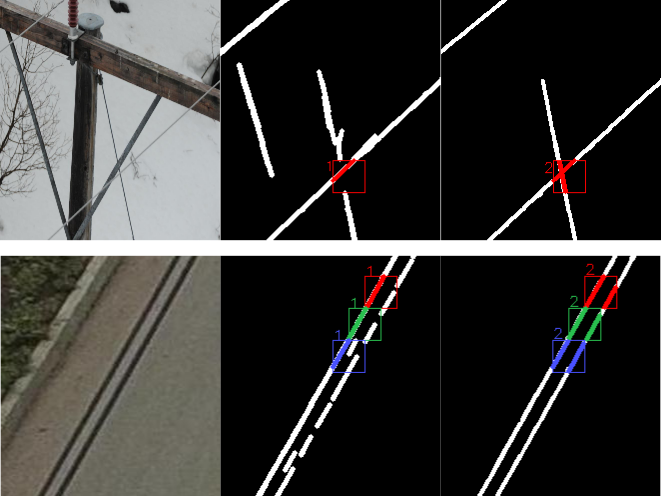
\includegraphics[width=\linewidth]{imgs/others/first.png}
  \caption{LSNet and the proposed LSNetv2 divide the images into grids and infer the existence and location of powerline segments in each grid cell. An example of a polyline, which is the path composed by multiple connected line segments, is shown in green in the image in the bottom row in the left column. LSNet can only output one prediction for each cell (middle column), thus, the combined output might miss some line segments, especially when multiple powerlines intersect and/or are in close proximity of each other. LSNetv2 has the capability to detect multiple line segments in each grid cell (right column) and, hence, is able to produce more complete powerline detections.}
  \label{first_examples}
\end{figure*}

% The very first letter is a 2 line initial drop letter followed
% by the rest of the first word in caps.
% 
% form to use if the first word consists of a single letter:
% \IEEEPARstart{A}{demo} file is ....
% 
% form to use if you need the single drop letter followed by
% normal text (unknown if ever used by the IEEE):
% \IEEEPARstart{A}{}demo file is ....
% 
% Some journals put the first two words in caps:
% \IEEEPARstart{T}{his demo} file is ....
% 
% Here we have the typical use of a "T" for an initial drop letter
% and "HIS" in caps to complete the first word.
Electricity is the lifeblood of modern society, thus, it is essential to ensure a stable electrical power supply across the nations. Hence, it is of utmost importance for utility companies to inspect and maintain their electrical facilities regularly. These tasks were conventionally done by human inspectors manually following, observing, and assessing the power grid \cite{9225728}. Recently, Unmanned Aerial Vehicles (UAVs) have been deployed to produce higher quality and more efficient observations due to their superior efficiency and ability to access higher altitudes and more hazardous environments \cite{Deng2014UnmannedAV}. Additionally, to enhance the effectiveness and efficiency of inspection and maintenance tasks, there has been an increased focus on automating the assessment step of the observations obtained by the UAVs, which, in many cases, are RGB camera images \cite{nhan_examples}. Towards this goal, several automatic assessment solutions have recently been proposed, many of which being fueled by the power of artificial intelligence and deep learning. Examples of such tasks are the detection of electrical components (insulators, cable suspension clamps, etc.) and the diagnosis of defects (pole breakage, insulator contamination, etc.) \cite{nhan_examples, insulator_examples,detect_component_examples}. Among these tasks, cable, wire, or powerline recognition and localization are very crucial as powerlines are one of the most essential elements in any utility infrastructure as they are directly responsible for electricity transmission. Accurate detection of powerlines can facilitate better analysis of faults (tears, kinking, bird caging, etc.) and identification of hazards (vegetation encroachment, etc.) on the powerlines. These tasks are extremely vital as their failure can lead to catastrophic and fatal consequences \cite{pge_bankruptcy}. Furthermore, the ability to detect powerlines is imperative for UAVs, and other forms of low-altitude flights, to navigate safely.

However, it is nontrivial to detect powerlines due to their inconspicuous appearances. Powerlines can be very thin and might be missed by proximity sensors on UAVs. Similarly, on camera images, the width of powerlines may only be a single pixel. Furthermore, cluttered backgrounds, occlusion, and same-colored backgrounds, such as white coating on snow, can cause the powerlines to be imperceptible. Other conditions, such as fog and lighting, can also negatively affect the discernability of powerlines on images. 

Towards automatic detection of powerlines, early methods utilize popular classical line segment detection methods \cite{related_work_kasturi_2002, related_work_guanjian_yan_2007, related_work_li_zhenrong_2010, related_work_candamo_2009, related_work_golightly_2005, related_work_zhengrong_li_2008, related_work_boris_alpatov_2016}. They rely on the assumption of clear visibility and straight line appearance of powerlines. However, these methods require intricate post-processing steps to distinguish between spurious lines and powerlines that can require expertise. Also, they are quite inaccurate and slow. 
More recently, facilitated by the increasing availability in data and hardware, deep learning has been gaining popularity
%due to their ability to directly extract robust features from data.. Deep learning can learn complex features and information directly from data without the help of expertise knowledge, which might be helpful yet can be lacking and biased. Deep learning approaches have achieved outstanding performance across many tasks and domains, 
for powerline detection. Several deep learning approaches have been proposed that frame the powerline detection task as semantic segmentation \cite{related_work_rainesh_mandaan_2017,related_work_heng_zhang_2019,related_work_yan_li_2019,related_work_rabab_abdelfattah_2022,related_work_rabeea_haffari_2021}. These methods can achieve quite competitive performance, however, gathering the pixel-level annotations required for these approaches is a big challenge, especially for objects with long and thin appearances like powerlines. This difficulty of producing pixel-level ground truth can be problematic, as in order to obtain a powerline detector that is effective and robust across various settings of input images (variations in lighting conditions, scenes, distances, powerline types, utility infratstructures, etc.) large amount of data should be procured. To address this problem, LSNet \cite{Nguyen2020} proposes to use polylines that trace the powerlines as ground truth (examples are shown in Fig. \ref{first_examples}). 
%The polyline annotations can be generated at considerably higher efficiency. The lack of width information in the ground truth will result in the detection method inferring no or imprecise width estimation of the powerlines. However, from our observation, the prediction of polylines or line segments tracing the powerlines is sufficient for inspection downstream tasks, which only requires the location to concentrate on.
These polyline annotations are cheaper to obtain, but can lead to imprecise width estimation of powerlines due to the lack of width information in the ground truth. However, our observations indicate that in many real-world settings, predicting polylines or line segments that trace the powerlines is adequate for downstream inspection tasks, as these primarily require accurate location information.

LSNet \cite{Nguyen2020} %was proposed to leverage this cheaper type of annotations. It 
is a Convolutional Neural Network (CNN) single-shot line segment detector that can be trained from polyline annotations. In LSNet, images are divided into overlapping grids and the detector leverages two output branches to first classify whether each cell grid has a line segment belonging to a powerline and second regress the endpoints of these line segments.
%. The other is a line segment regressor to locate the endpoints of these line segment. 
However, LSNet has several limitations. One major constraint is that LSNet only is able to detect and locate one line segment in each grid cell. While this design allows LSNet to obtain good performance on simpler datasets, where the powerlines are arranged relatively far apart and not intersecting with each other, its design limits its application in more practical settings, where the powerlines can appear visually to be of very close proximity or to cross each other resulting in cases where there are multiple line segments in a single cell. This is illustrated in Fig. \ref{first_examples}.In addition, LSNet struggles to effectively detect more concealed line segments and discern spurious lines due to its limited ability to reason over extended image regions  due to its small receptive field. Furthermore, the regression loss used to train the localization capability of LSNet can introduce training instabilities due to LSNet's swap mechanism that introduces an interdependence between the predicted endpoints of the line. %where confusion by not concretely define the inference responsibility of each output elements.}
% stemming from its relatively small receptive field.} the backbone of LSNet has a relatively small receptive field, which is not effective in gathering non-local semantics across the entire input image to help in detecting more concealed line segments.

In this paper, we propose an improved version of LSNet, aptly named LSNetv2, to address to aforementioned problems. First, to efficiently detect powerline crossings and powerlines that are in close proximity, we provide LSNetv2 with the capability to detect multiple line segments. This is facilitated by allowing the model to make multiple predictions on each divided cell location and leveraging a bipartite matching loss for training. In addition, to eliminate the interdependence of the line endpoints during line segment localization, we also modified the loss for the regression branch of LSNet by fixing the ordering of the endpoints. Finally, to increase the potency of LSNetv2 as well as to provide it with the ability to obtain global information, we replace the backbone from the original modified-VGG16 \cite{vgg} to a model from the state-of-the-art ConvNext family \cite{convnext} that provides a larger receptive field to the detector. We empirically demonstrate the benefit of LSNetv2 on a wide-range of powerline detection tasks, illustrating its superiority over LSNet.



% An example of a floating figure using the graphicx package.
% Note that \label must occur AFTER (or within) \caption.
% For figures, \caption should occur after the \includegraphics.
% Note that IEEEtran v1.7 and later has special internal code that
% is designed to preserve the operation of \label within \caption
% even when the captionsoff option is in effect. However, because
% of issues like this, it may be the safest practice to put all your
% \label just after \caption rather than within \caption{}.
%
% Reminder: the "draftcls" or "draftclsnofoot", not "draft", class
% option should be used if it is desired that the figures are to be
% displayed while in draft mode.
%
%\begin{figure}[!t]
%\centering
%\includegraphics[width=2.5in]{myfigure}
% where an .eps filename suffix will be assumed under latex, 
% and a .pdf suffix will be assumed for pdflatex; or what has been declared
% via \DeclareGraphicsExtensions.
%\caption{Simulation results for the network.}
%\label{fig_sim}
%\end{figure}

% Note that the IEEE typically puts floats only at the top, even when this
% results in a large percentage of a column being occupied by floats.


% An example of a double column floating figure using two subfigures.
% (The subfig.sty package must be loaded for this to work.)
% The subfigure \label commands are set within each subfloat command,
% and the \label for the overall figure must come after \caption.
% \hfil is used as a separator to get equal spacing.
% Watch out that the combined width of all the subfigures on a 
% line do not exceed the text width or a line break will occur.
%
%\begin{figure*}[!t]
%\centering
%\subfloat[Case I]{\includegraphics[width=2.5in]{box}%
%\label{fig_first_case}}
%\hfil
%\subfloat[Case II]{\includegraphics[width=2.5in]{box}%
%\label{fig_second_case}}
%\caption{Simulation results for the network.}
%\label{fig_sim}
%\end{figure*}
%
% Note that often IEEE papers with subfigures do not employ subfigure
% captions (using the optional argument to \subfloat[]), but instead will
% reference/describe all of them (a), (b), etc., within the main caption.
% Be aware that for subfig.sty to generate the (a), (b), etc., subfigure
% labels, the optional argument to \subfloat must be present. If a
% subcaption is not desired, just leave its contents blank,
% e.g., \subfloat[].


% An example of a floating table. Note that, for IEEE style tables, the
% \caption command should come BEFORE the table and, given that table
% captions serve much like titles, are usually capitalized except for words
% such as a, an, and, as, at, but, by, for, in, nor, of, on, or, the, to
% and up, which are usually not capitalized unless they are the first or
% last word of the caption. Table text will default to \footnotesize as
% the IEEE normally uses this smaller font for tables.
% The \label must come after \caption as always.
%
%\begin{table}[!t]
%% increase table row spacing, adjust to taste
%\renewcommand{\arraystretch}{1.3}
% if using array.sty, it might be a good idea to tweak the value of
% \extrarowheight as needed to properly center the text within the cells
%\caption{An Example of a Table}
%\label{table_example}
%\centering
%% Some packages, such as MDW tools, offer better commands for making tables
%% than the plain LaTeX2e tabular which is used here.
%\begin{tabular}{|c||c|}
%\hline
%One & Two\\
%\hline
%Three & Four\\
%\hline
%\end{tabular}
%\end{table}


% Note that the IEEE does not put floats in the very first column
% - or typically anywhere on the first page for that matter. Also,
% in-text middle ("here") positioning is typically not used, but it
% is allowed and encouraged for Computer Society conferences (but
% not Computer Society journals). Most IEEE journals/conferences use
% top floats exclusively. 
% Note that, LaTeX2e, unlike IEEE journals/conferences, places
% footnotes above bottom floats. This can be corrected via the
% \fnbelowfloat command of the stfloats package.
\begin{figure*}[hbt!]
  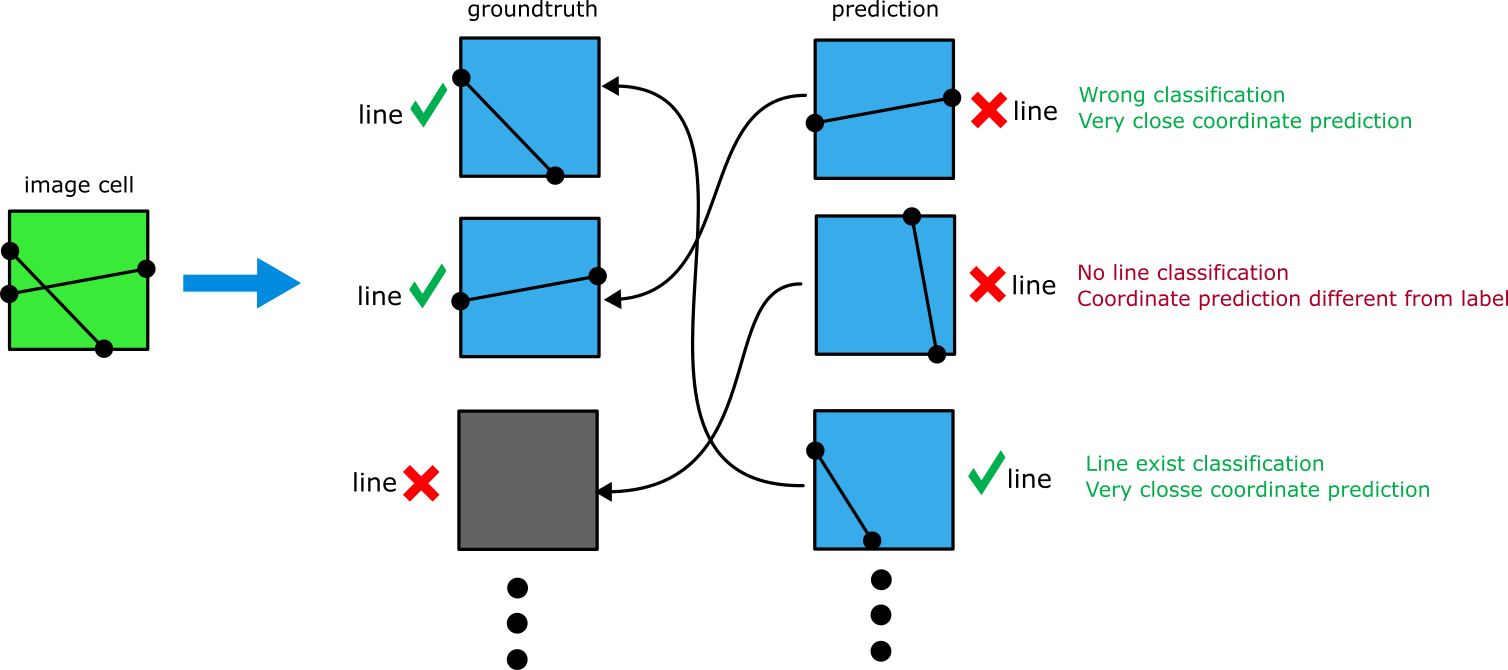
\includegraphics[width=\linewidth]{imgs/others/bimatching.png}
  \caption{Illustration of the bipartite matching mechanism that facilitate the multi-guess capability of LSNetv2. The multiple predictions of each cell are matched to the multiple groundtruths based on its classification and localization of endpoints.}
  \label{bimatching}
\end{figure*}


\section{Related Work}

The problem of powerline detection has been tackled with traditional computer vision and more recently with deep learning approaches. In this section, we briefly review the most prominent and related approaches.

\subsection{Traditional powerline detection approaches}

A notable early attempt of powerline detection was proposed by Kasturi et al. \cite{related_work_kasturi_2002}, where Steger's method \cite{related_work_steger_1998} was used to extract features, which are then filtered using the Hough transform to exclude short lines. Yan et al. \cite{related_work_guanjian_yan_2007} proposes instead to leverage the Radon transform to generate line segments, group these segments by slope and distance thresholding, and then finally use Kalman filters as a post-processing step. Li et al. \cite{related_work_li_zhenrong_2010} remove clutter and noise in the background using a pulse coupled neural filter before using Hough transforms and K-means clustering to detect and combine line segments. However, the aforementioned solutions and similar works~\cite{related_work_candamo_2009, related_work_golightly_2005, related_work_zhengrong_li_2008, related_work_boris_alpatov_2016} hold the strict assumptions that powerlines appear straight and have parallel orientations, and thus, do not always apply in reality. Song et al. \cite{related_work_biqin_song_2014} aimed to address this problem and were able to detect curved powerlines by using a normalized graph cut model to link line segments, which were produced from the responses of a matched filter and first-order derivative of a Gaussian. However, all of these traditional approaches are severely affected by the conditions in which the input images were taken. Any differences in camera settings, environment, lighting, and view angle requires extensive tuning of hyper-parameters of these methods and require specialist expertise.

\subsection{Deep learning based approaches}
Deep learning aims to alleviate the problems of the abovementioned traditional computer vision approaches. With enough data, deep learning solutions for classification and detection can generalize well to different acquisition conditions. Pan et al. \cite{related_work_chaofeng_pan_2016} suggest training a CNN that takes in edge features, which are produced by steerable filters, and classifies whether square patches from an input image contains a line or not. Then the Hough transform is used to detect the powerline segments. Similarly, Gubbi et al. \cite{related_work_jayavardhana_gubbi} also propose using a CNN but, instead, use Histogram of Oriented Gradient features as input. The line segment detector proposed in \cite{lsd} was used as a post-processing step. Since the inputs of these two methods are individual patches, the CNN models lack the contextual information of the entire images. Hence the performance can be limited, especially for low-contrast images with a cluttered background. Yetgin et al. \cite{related_work_omer_emre_yetgin_2018} finetuned a CNN, which was pretrained on ImageNet \cite{deng2009imagenet} via two methods. One is with a newly initialized linear layer with softmax that classifies the powerline existence and is trained jointly with the feature extractor. The other method is to use dimension-reduced features from immediate layers of the pre-trained CNN to train a classifier separately. However, these two proposed methods only detect the existence of powerline for real-time warning systems without localization. More recent approaches \cite{related_work_rainesh_mandaan_2017,related_work_heng_zhang_2019,related_work_yan_li_2019,related_work_rabab_abdelfattah_2022,related_work_rabeea_haffari_2021} frame powerline detection as binary pixel-level classification problems where each pixel is classified whether is belongs to the powerline or not. This type of problem can be undertaken by deep learning semantic segmentation networks. Madaan et al. \cite{related_work_rainesh_mandaan_2017} investigate different dilated convolutional neural networks for segmenting powerlines. Zhang et al. \cite{related_work_heng_zhang_2019} produce segmentation by fusing hierarchical feature maps from each layers of a VGG-16 model \cite{vgg} as well as structure features, such as powerline length, width and orientation. In \cite{related_work_yan_li_2019}, a CNN is introduced with two components: an information fusion module and an attention module. The information fusion module is in an encoder-decoder structure, where decoding stages are combined with their corresponding same-scaled encoding stages to fuse semantic and location information for accurate powerline segmentation. The attention module produces, from the last feature map of the encoder, a weight map, which is multiplied elementwise with the decoder output to increase more focus on regions with powerlines. Abdelfattah et al. \cite{related_work_rabab_abdelfattah_2022} trained a Generative Adversarial Network (GAN) to generate modified versions of the input images where the powerlines are highlighted. A semantic decoder connected to an immediate layer of the generator is also trained jointly in order to perform the actual segmentation task. Jaffari et al. \cite{related_work_rabeea_haffari_2021} introduce a new type of focal loss based on Phi coefficient \cite{phi_coeff} to improve powerline segmentation performance of U-Net\cite{unet}-based architectures. These semantic segmentation methods have achieved satisfying results, however, they require training data with pixel-level annotation, which can be laborious to obtain.  Especially in the case of powerlines, which can often be quite slender yet span across images, and require meticulousness in the annotating process. Lee et al. \cite{related_work_sang_jun_lee_2017} aims to mitigate this burden by relying only on image-level annotation from patches, which are extracted from the input images via sliding windows, to train a CNN to classify the existence of powerline segment in patches of input images. Visualization of positive patches is performed using the Visualbackprop algorithm \cite{vbp} to achieve localization. The visualizations are performed on multiple layers of the network and are merged together via bilinear interpolation and multiplication. Choi et al. \cite{related_work_hyeyeon_choi_2021} also used image-level annotation to train classification CNN for patches on the input images. Visualbackprop visualization is performed to approximate pseudo segmentation so that another fully convolutional network can be trained trained to perform segmentation. However, while reducing the labelling effort required, these approaches have been reported to have low performance \cite{choi_low_evidence} due to among others the sliding window mechanism that restricts the integration of global context when considering a given patch.

The predecessor of our proposed method, LSNet, reduces the need for expensive and labor-intensive pixel-level annotations by only relying on polyline annotations that traces along the powerline. Polyline annotation requires much less effort and are arguably more robust to labeling inaccuracy allowing more ground-truth images to be acquired and facilitating better deep learning models. LSNet is trained to detect and locate small line segments within the ground truth polylines, which are divided by four overlapping grids. LSNet is quite competitve in the powerline detection task, however, it is unable to detect powerlines that are in close proximity or appear to intersect each other. This drawback leads to LSNet not being able to guarantee the complete the detection of all powerlines as illustrated in Fig. \ref{first_examples}.

While not directly addressing the powerline detection problem, recent work has been conducted on addressing the wireframe parsing problem, which shares certain similarities. The wireframe parsing problem aims to find the boundary of objects, structures, and regions in the form of line segments and corresponding end-points for geometric reasoning. L-CNN \cite{lcnn} infer the endpoints in an end-to-end manner. From these points, proposed line segments are sampled and verified with a line of interest pooling layer (LoiPooling) that took inspiration from RoIPool \cite{fastrcnn} and RoIAlign \cite{maskrcnn} layers from the object detection. HAWP \cite{hawp} transforms the original line segment labels into Holistic Attraction Fields (HAT) where each pixel is parameterized based on its position in relation to its closest line segments. A model is trained to approximate these fields, from which line segments can be derived. HAWPv2 \cite{hawpv2} combined the strengths of LoiPooling and HAT, along with some new techniques, to improve the performance. While the adaption of wireframe approaches to the powerline detection problem is promising, we demonstrate empirically that a direct application of these methods leads to sub-optimal results. 

\begin{figure}
  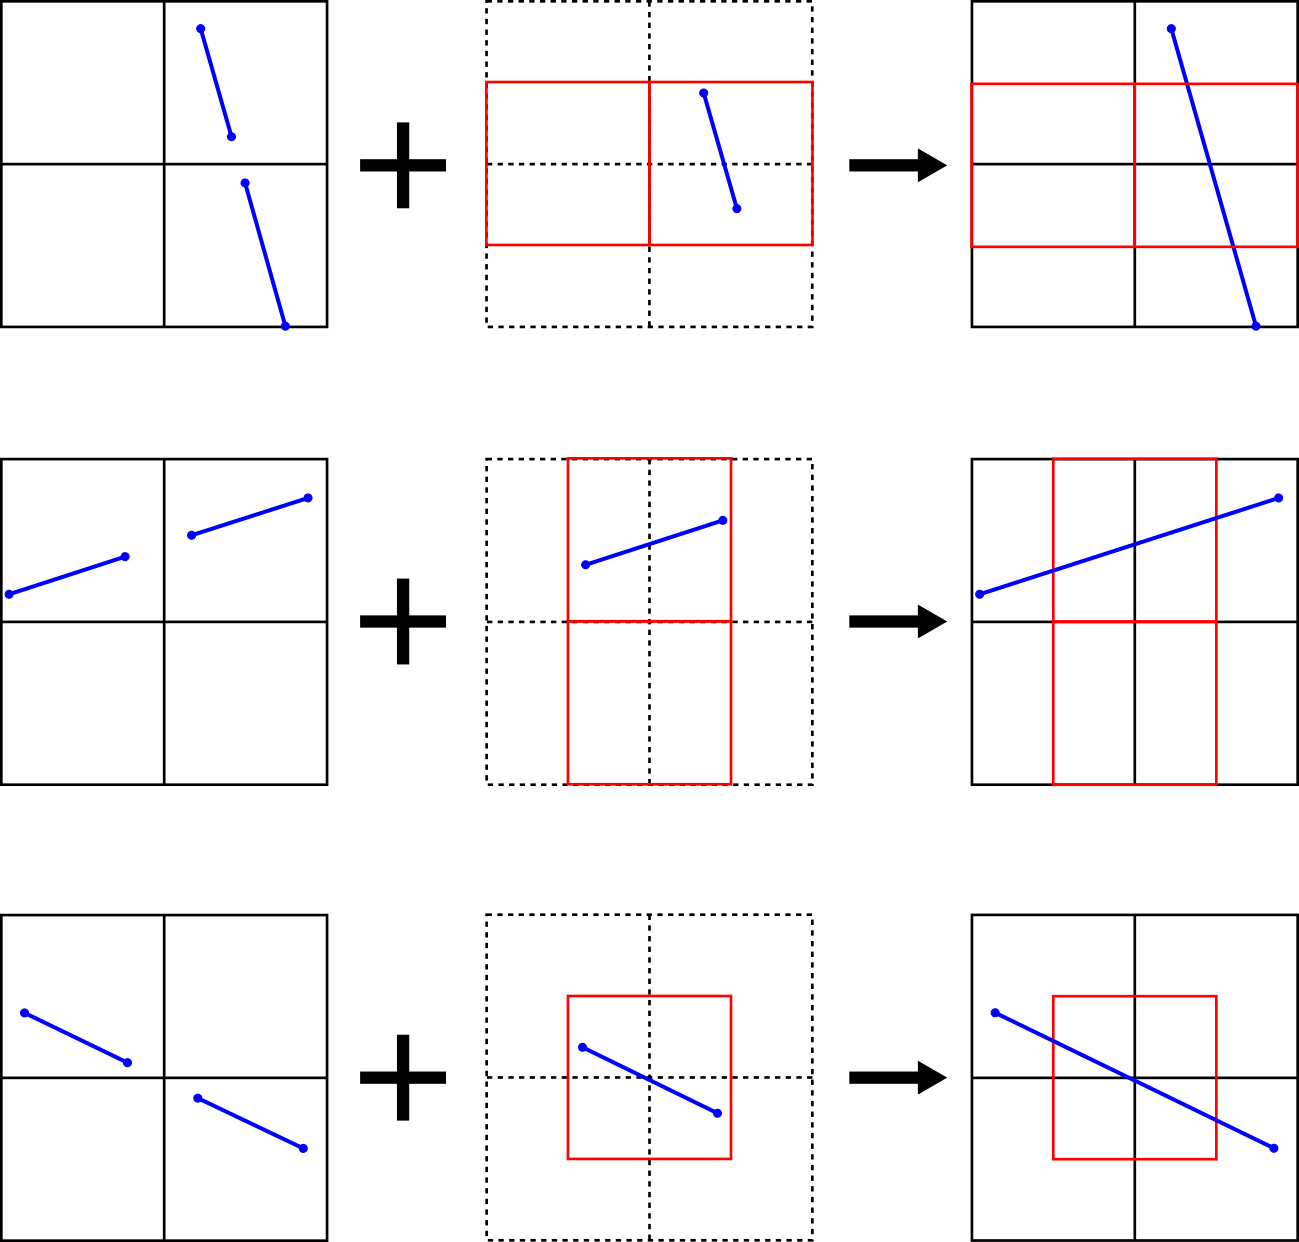
\includegraphics[width=\linewidth]{imgs/others/new_4grid.png}
  \caption{Depiction of the for-grid approach. With one grid like the first column, LSNet face the problem of disconnection at the border and corner of cells. By utilizing additional three grids (second column), the gaps can be close and LSNet can provide more complete detections of powerlines.}
  \label{4grid}
\end{figure}

\section{Methodology}

In this section, we first give a short description of LSNet and highlight its shortcomings. After that, we introduce the design of LSNetv2 and detail how it addresses these limitiations.

\subsection{Preliminaries: LSNet}
LSNet \cite{Nguyen2020} was proposed as a single-shot line-segment detector inspired by SSD \cite{SSD} and YOLO \cite{YOLO}. Specifically, LSNet breaks down the problem of powerline detection into detecting and locating line segments in four overlapping grids, which are superimposed onto the input image. For the case of input images having the size of $512 \times 512$, this results in a grid of $31 \times 31$ cells, each of which overlooks an area of size $32 \times 32$ in the image. For each cell of the grids,  LSNet detects whether there exist parts of powerlines within its borders and provides the coordinates of the line segment endpoints. These divided results can be combined to produce a complete segment map of powerlines. The four-grid approach was proposed as opposed to the one-grid approach, commonly found in models such as SSD and YOLO, in order to encourage more thorough detection and localization of powerlines and combat the problem of discontinuities at grid cell borders and corners. This is illustrated in Fig. \ref{4grid}. 

To perform line segment detection, the architecture of LSNet involves a fully convolutional feature extractor (backbone) which branches out into a classifier module and a regressor module. These two modules aim to detect the presence of a line segment and the line segment endpoint coordinates respectively. The classifier module and regressor module shared a similar design and have the output of shape $B \times 31 \times 31 \times 2$ and $B \times 31 \times 31 \times 4$ respectively, with $B$ being the batch size. The $B \times 31 \times 31$ vectors from the classification module determine if line segments exist in their corresponding cells and the $B \times 31 \times 31$ vectors from the regression module determine the xy-coordinates of the endpoints of the line segments. This design leads to LSNet being able to only detect the existence and location of one line segment per cell and, thus, may not be effective in cases where more than one line segment existing in cells, such as when powerlines appear to be in close vicinity or cross each other. 

The classifier and regressor modules are trained with Focal loss \cite{focal_loss} and Wing loss \cite{wing_loss} respectively (more details are given in \ref{lsnetv2_subsection}). The distance error, which is used for the Wing loss, is defined as the minimum $L_1$ loss between the ground truth pairs and the predicted pairs, where the predicted pairs are permuted to result in the minimum loss. We observe that this premutation can lead to training instabilities when training LS-Net, caused by the predictions being interdependent, resulting in sub-optimal results.

The feature extractor of the original LSNet was proposed to be a version of VGG-16 network \cite{vgg} which was modified to include Group Normalization \cite{group_norm} before the activation functions and all max pooling layers where replaced by leveraging a stride of 2 in the convolutional layers. 
%This architecture might not be an effective backbone as it does not possess recent advancements in deep learning. 
This architecture leads to a relatively small receptive field,  only covering an area of about four times the size of a cell, resulting in inconsistent detections when context information is required, as for instance when a powerline is blending in with the background.




\subsection{LSNetv2}\label{lsnetv2_subsection}
In this section, we introduce our proposed LSNetv2, which aims to address the abovementioned limitations of LSNet.
%As aforementioned, in practice, images captured for inspection commonly have powerlines visually intersecting or being in close proximity to each other. Even though, with LSNet, images are well divided into cells, it is expected that there are cells where there are multiple line segments line segments which can not be ignored when trying to model powerlines in their completeness in order to facilitate effective visual inspection down the line. Thus, LSNet, being able to only detect one line segment per cell, is lacking. 
In practice, images captured for inspection commonly have powerlines visually intersecting or being in close proximity to each other, which LSNet is unable to model.
We therefore design LSNetv2 to detect multiple lines per cell by performing a fixed number of inferences N, which are chosen to be larger than the maximum number of line segments that are believed to exist in the cell. From our observations, $N=10$ is a safe choice. This results in the output of the classification and regression being in the shape of $B \times 31 \times 31 \times N \times 2$ and $B \times 31 \times 31 \times N \times 4$, respectively (Fig. \ref{lsnet_architecture}). For ease of notation, we in the following focus the scope of our discussion on an individual cell. The ground truth $y$ of each cell, which contains $m$ actual line segments, is also perceived to contain $N$ line segments $y=\{y_i\}^N_{i=1}$. However, the ground truth is now padded with $N-m$ negative classification. Inspired by DETR \cite{DETR}, we frame the line segment detection within each cell as a direct set prediction problem. In our loss computation step, we include an optimal bipartite matching between the $N$ predictions and $N$ ground truths.

\begin{figure}
  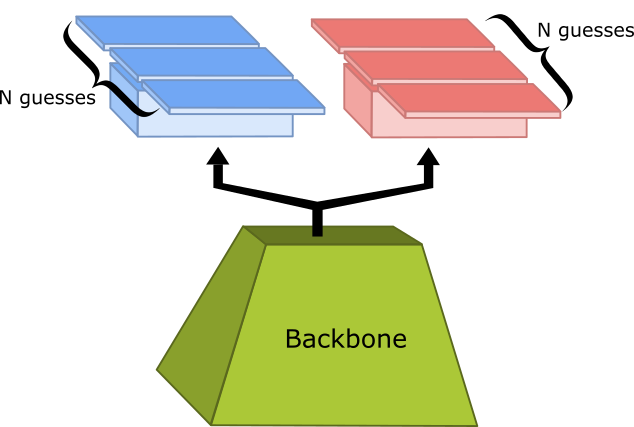
\includegraphics[width=\linewidth]{imgs/others/lsnet_arch.png}
  \caption{LSNetv2 shares similar overall design as LSNet with a fully convolutional feature extractor, a classifier module and a regressor branch module. However, the two branches now perform multiple guesses so that LSNetv2 has the capability to detect multiple line segment per cell.}
  \label{lsnet_architecture}
\end{figure}

Let $\hat{y}=\{\hat{y}_i\}^N_{i=1}$ be the set of $N$ predictions. The optimal bipartite matching between the $N$ predictions and $N$ ground truths, which is done using the Hungarian algorithm, produces a permutation $\hat{\sigma} \in \mathfrak{S}$ that satisfies:

\begin{equation} \label{bipartite_eqn}
\hat{\sigma} = \mathop{\arg \min}\limits_{\sigma \in \mathfrak{S}} \sum_{i=1}^N \mathcal{L}_{match} (y_i, \hat{y}_{\sigma(i)})
\end{equation}

\noindent where $\mathcal{L}_{match} (y_i, \hat{y}_{\sigma(i)})$ is the loss when pairing $y_i = (c_i, b_i)$ and $\hat{y}_{\sigma(i)} = (\hat{p}_{\sigma(i)}, \hat{b}_{\sigma(i)})$, which is reordered via permutation $\sigma(i)$. Similarly to \cite{DETR}, this loss is defined as $-\hat{p}_{\sigma(i)}(c_i) + L_1(b_i, \hat{b}_{\sigma(i)})$, where $b_i$ and $\hat{b}_{\sigma(i)}$ are line segment endpoint ground truth and permutated prediction at index $i$ respectively. $L_1(.)$ is the $L_1$ loss and $\hat{p}_{\sigma(i)}(c_i)$ is the predicted probability of class $c_i$, which is the classification ground truth at index $i$. The permutation $\hat{\sigma}$ is found by solving the linear sum assignment problem with a modified Jonker-Volgenant algorithm \cite{7738348}.

After bipartite matching has been done, the model can be trained with a multitask loss, $\mathcal{L}$, to simultaneously train the classification and regression module:

\begin{equation} \label{multitask_training_loss}
\mathcal{L} = \sum_{i=1}^N\mathcal{L}_{\text{cls}}(y_i, \hat{y}_i) + \lambda \sum_{i=1}^N\mathds{1}_{\{c_i=\text{positive}\}}\mathcal{L}_\text{reg}(y_i, \hat{y}_i) 
\end{equation}
\noindent where $\hat{y}_i = \hat{y}_{\hat{\sigma}(i)}$ is one of $N$ prediction at an arbitrary cell after bipartite matching. $\mathcal{L}_{\text{cls}}$ is a Focal loss \cite{focal_loss}:
\begin{equation}
  \mathcal{L}_{\text{cls}} =
    \begin{cases}
      -\alpha (1 - p)^\gamma \log(p) \text{,  if  } c_i=\text{positive} \\
      -(1 - \alpha)p^\gamma \log(1-p) \text{,  otherwise} 
    \end{cases}       
\end{equation}

\noindent where $p=\hat{p}_{\hat{\sigma}(i)}(\text{positive})$, $\alpha \in [0, 1]$ and $\gamma \geq 0$ are tunable hyperparameters that adjust the weight on uncommon class and misclassified examples respectively. This loss is used in the original LSNet to tackle the imbalance problem between cells with line segments and cells without. In LSNetv2, we continue to use this loss to train the classification module.

The regression module is trained using the Wing loss \cite{wing_loss} so that the training is more sensitive to small errors and robust against outliers. The loss is defined as:

\begin{equation}
  \mathcal{L}_{\text{reg}} =
    \begin{cases}
      w \text{ln} (1 + \frac{d}{\epsilon}) \text{, if } d < w \\
      d - C \text{,  otherwise}
    \end{cases}       
\end{equation}

\noindent where $w$ is used to constrain the range of the nonlinear behavior of the loss to $(-w, w)$, $\epsilon$ controls the growth of loss as regression error increases and the curvature of the nonlinear part, $C = w - w\text{ln}(1 + w / \epsilon)$ is used to smoothen the connection between the linear and nonlinear parts of the loss, and $d$ is the distance error. 
With $b_i = (b_i^{x_1}, b_i^{y_1}, b_i^{x_2}, b_i^{y_2})$ and $\hat{b}_i = \hat{b}_{\hat{\sigma}(i)} = (\hat{b}_i^{x_1}, \hat{b}_i^{y_1}, \hat{b}_i^{x_2}, \hat{b}_i^{y_2})$, the distance error for the original LSNet was defined as:

\begin{equation}
  d_{\text{LSNet}}(b_i, \hat{b}_i) = \min(\sum (|b_i - \hat{b}_i|), \sum(|b_i - \text{swap}(\hat{b}_i)|))
\end{equation}

\noindent where $\text{swap}(\hat{b}_i) = (\hat{b}_i^{x_2}, \hat{b}_i^{y_2}, \hat{b}_i^{x_1}, \hat{b}_i^{y_1})$.

However, we observe that the swapping mechanism, which allows the a value pair in the regression module to predict the location of an arbitrary endpoint based on its closeness to the ground truth introduces unwanted interdependence between the endpoints, resulting in training instabilities. Specifically, during training, the prediction of one endpoint relies on the position and closeness of the other point to either of the groundtruth endpoints, which can lead to changes in groundtruth-prediction assignment and thus inconsistent updates.
%and the switching can cause the prior part of the training process, which aims to predict the original endpoints, to be meaningless or less effective. 
Thus, for LSNetv2, we propose the ordered distance error as follows:
\begin{equation}
  d_{\text{LSNetv2}}(b_i, \hat{b}_i) = \sum (|b^*_i - \hat{b}_i|)
\end{equation}

\noindent where 

\begin{equation}
  b^*_i=
    \begin{cases}
       (b_i^{x_1}, b_i^{y_1}, b_i^{x_2}, b_i^{y_2}) \text{, if } b_i^{x_1} < b_i^{x_2} \\
       (b_i^{x_2}, b_i^{y_2}, b_i^{x_1}, b_i^{y_1}) \text{, otherwise }
    \end{cases}       
\end{equation}

This distance error ensures that the endpoints with the lower x-coordinate and the endpoints with the higher x-coordinate are detected by the same output elements in the 4-element vectors output from the regression module. With this restriction, the training process is more robust and we empirically demonstrate the performance improvement in the experiment section.
%, the new ordered regression loss with this distance error helps improve the performance of LSNetv2.




% \textcolor{brown}{We propose a new version of LSNet, called LSNetv2. This version is updated with recent advancements in the deep learning space. \commentM{Again, here it sounds like you "just" leverage a new backbone and other new things. Motivate it instead from the problem and then the solution is a method that incorporates new components.}
% Specifically, the feature extractor is altered with the state-of-the-art ConvNext model. Furthermore, inspired by DETR \cite{DETR}. LSNetv2 possess the ability to detect and locate multiple line-segments within each grid cell via multi-guess bipartite matching.  \textcolor{red}{Also, we propose the addition of a context module built from multi-head attentions layers, whose effectiveness in extracting global information has been proven}. Finally, \textcolor{red}{adjustments are made to the losses so that the training is more stable and requires less time to achieve plateau performance}.}

It has been shown that LSNet has been successful for cases where images of powerlines are captured from a relatively close distance and the visibility of the powerlines throughout the span of the image is clear \cite{Nguyen2020}. However, in most practical application settings, images such as those used for visual inspection are taken from further away leading to segments of powerlines appearing thin and/or blending in with the background. Following the grid-based approach of LSNet, the detection performance of powerlines in each cell, especially ones that are inconspicuous, may depend heavily on the global information of areas around it. However, the theoretic receptive field of LSNet is only about four times the cell size. %(91 as calculated by \texttt{receptive\_field\_analysis\_toolbox} \cite{receptive_field_analysis_toolbox}). 
This limits the capability of LSNet to aggregate global context for the cell inference.  Thus, LSNetv2 is designed to have a larger receptive field. In particular, we leverage the ConvNext-Tiny backbone, which increases the receptive field by a factor of 12. %(also calculated via calculated by \texttt{receptive\_field\_analysis\_toolbox}).
ConvNext-Tiny, which is the smallest in the ConvNeXt, was recently introduced as a modernized version of ResNet \cite{resnet} which is equipped with recent properties based on the hierarchical vision transformer Swin \cite{swin}. 
%Iterative modifications were made to ensure that ConvNext-Tiny, and others in the ConvNeXt family, competes favorably with other architectures, including Swin, which is among the state-of-the-art for deep vision tasks. 
We use an altered version of ConvNeXt-Tiny. Similarly to ResNet and other well-known CNNs, ConvNext-Tiny has a multi-stage design of 4 stages. Each stage results in the compression of the features with the compression ratio of 2. We use a ConvNeXt-Tiny, which is truncated before the compression layer of the 3rd stage, as the new backbone. The output of the truncated model reduces the input to a size of 32x32x384. %Using ConvNext-Tiny, LSNetv2 has a theoretical receptive field of 1096. 
The architecture is detailed in Table \ref{backbone_arch}.

\subsection{Implementation Details}
The proposed LSNetv2 is implemented in Tensorflow. Each model is trained on one NVIDIA RTX 3090 24GB. The model was initialized using Xavier initialization \cite{xavier} and trained with a batch size of 8 for 100 epochs. The Adam optimizer \cite{adam} is used with a learning rate of 0.0001, the first momentum of 0.9, and the second momentum of 0.99. The input image size is 512 x 512. During training, augmentation techniques applied include randomized occurrences of sharpening, blur, color jittering, pixel dropouts, and additive noise. After that, randomized square crops of varying sizes between 360 and 512 are taken from the input and then scaled back to the input size of 512 x 512.

\section{Experiments}
%The procedure and results of the experiments are presented. Comparisons to state-of-the-art are also conducted. 
In this section, we provide quantitative and qualitative evaluations of our proposed approach and illustrate its advantages over the current state-of-the-art approaches LSNet~\cite{Nguyen2020} and HAWPv2 \cite{hawpv2}. HAWPv2 is included in the comparsion as it can be can be considered the state-of-the-art approach for wireframe parsing. It is an improved version of the highly-cited HAWP and, to the best of our knowledge, HAWPv2 achieved the highest performance in popular wireframe parsing benchmarks. As mentioned above, wireframe parsing is, in essence, very similar to the task of powerline detection and HAWPv2 can be trained directly with the polyline annotations. Experiments are conducted on four different powerline detection datasets of varying creation methods and difficulty. In addition, an analysis of different backbones was performed and ablation studies were done to highlight the benefit of the novel components that constitute LSNetv2, namely the multi-guess capability via bipartite matching, the ordered regression loss, and the new ConvNext-Tiny backbone.

\subsection{Datasets}

\subsubsection{PLD-UAV}

PLD-UAV \cite{PLD_UAV} contains two datasets of powerlines: the power line dataset of urban scenes (PLDU) and the power line dataset of mountain scenes (PLDM). In these datasets, the backgrounds are urban and mountain scenes respectively, and are relatively cluttered and complex. However, the powerlines to be detected are still quite observable. In this dataset, the boundaries of powerlines are annotated at the pixel level. To adapt to LSNetv2, we detected individual boundaries by dilating the pixel annotations and clustering the pixels via connected component analysis. From each cluster of pixels, a polygon is approximated and filled up with white pixels (positive labels). Then, a skeletonization algorithm, introduced in \cite{skeleton}, is used to produce polylines tracing the powerlines. The polylines are simplified using the Ramer–Douglas–Peucker (RDP) algorithm~\cite{RDP} and imposed on the 31x31 grid to produce the annotation for LSNetv2. Manual inspection was done to ensure that the procedure produces accurate labels. PLDU contains 453 training data points and 120 testing data points. PLDM contains 237 training data points and 50 testing data points.

\subsubsection{TTPLA}

TTPLA \cite{TTPLA} is a newly introduced dataset. It consists of images taken from UAVs under a variety of conditions, such as different scenes, angles, zoom, and lighting conditions. Many instances in this dataset suffer from problems like occlusion and blending, which make the detection more challenging. The annotation of TTPLA is provided at an instance segmentation level via polygons that precisely wrap around the power lines. TTPLA also possesses some data points that have powerlines being close to each other and powerline crossings. This makes it an ideal test bed to evaluate the effectiveness of our proposed method, which is designed to effectively segment multiple powerlines/line segments. To adapt this dataset to LSNetv2, similarly to the datasets above, we performed an image processing procedure that includes skeletonizing the blobs that fill the polygon annotations to generate polylines. The polylines are simplified using the RDP algorithm and then imposed on the 31x31 overlapping grid to find intersections, which are the labels for LSNetv2. This dataset contains 1242 images and we use 992 for training and 250 for testing.

\subsubsection{Esmart dataset}
We also evaluated the method using a proprietary dataset of powerlines aggregated by EsmartSystems \cite{esmart_website}. This dataset is made from UAV images taken by multiple clients of EsmartSystems, and thus, contains significant diversity in terms of scenes, angles, zooming levels, weather, and lighting conditions. This dataset has polyline annotations tracing the trajectories of the powerlines. The polyline annotation can be imposed onto the 31x31 grid to produce the annotation for LSNetv2.
In this dataset, the lines annotated include conductors, guy wires, and overhead ground wires. Conductors are normally in parallel. However, the other two types of wires can have different directions and, hence, there are many visual crossings. Included in the dataset are also some instances of line segments being in close proximity. The dataset contains 2961 images for training and 468 images for testing.


\subsection{Evaluation Metrics}\label{evaluation_metrics}
For comparison purposes, we follow prior work \cite{Nguyen2020} and evaluate LSNetv2 in the same manner as segmentation models.
Similarly to \cite{Nguyen2020}, we adopt pixel-level Averaged Recall Rate (ARR), Averaged Precision Rate (APR), and $F_1$ Scores. In addition, we also use averaged $F_{\beta}$:
\begin{equation}
  F_{\beta} = \frac{1}{N} \sum_{i=1}^N  \frac{(1 + \beta^2)\text{Precision} \times \text{Recall}}{\beta^2 \times \text{Precision} + \text{Recall}} 
\end{equation}
where $N$ is the number of test images and $\beta^2 = 0.3$ in order to place more emphasis on precision compared to the conventional $F_1$ metric. According to \cite{f_beta0, f_beta1}, recall is not as relevant as precision since the recall rate of 1.0 can be achieved by predicting all pixels in the image as positive. Also, %in the case of LSNetv2 
higher recall rates can be an indication of imprecise predictions of line segment endpoints as illustrated in Fig \ref{hirecall}. Thus the $F_{\beta}$ score can be considered a better measurement of the overall performance than the $F_1$ score.

To produce the segmentation map, for each cell within the 31x31 output grid that was classified to contain segments of powerlines, we use OpenCV to generate visible white lines from the predicted pairs of endpoints. Specific line widths are chosen for each dataset based on the common width of powerlines for each dataset. Through inspection, we find that the common width of the powerlines in PLDU dataset is 9. The average is 6 for PDLM dataset, 2 for TTPLA dataset, and 5 for Esmart dataset. 
%At these chosen widths, it is observed that the LSNetv2 was able to achieve competitive $F_{\beta}$ score.

\begin{figure}
  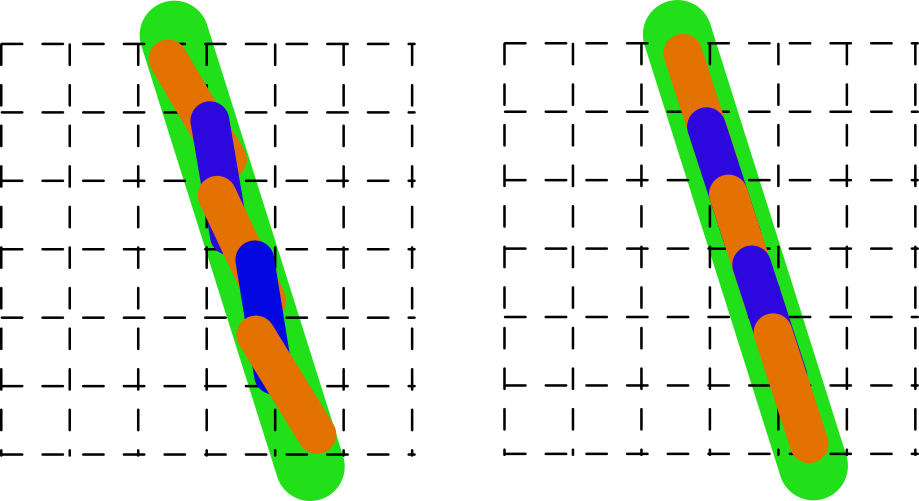
\includegraphics[width=\linewidth]{imgs/others/why_f_beta.png}
  \caption{Illustration of cases where imprecise inferences from LSNetv2 can leads to better reccall. The orange and blue segments are individual inferences of the cells. The line segment inferences are rasterized with a width. The green line are the ground truth rasterized with the actual line width. The left image shows that, especially in cases where the chosen line width is less than the actual one, imprecise inferences of line segments, when combined together, can include more true positive pixels without increase false positive pixels than the more precise inferences shown on the right.}
  \label{hirecall}
\end{figure}

\subsection{Evaluation Methods}

The comparison is done with the previously proposed LSNet across the four datasets. We also compare LsNetv2 with HAWPv2 by training the model, whose code is provided by the original author \cite{hawpv2code}, the output of HAWPv2 model is rasterized into segmentation maps, from which APR, ARR, $F_1$ and $F_\beta$ score are calculated. 
% \commentM{The following paragraph can probably be removed (as it is not really part of "evaluation methods".}
% In addition, an ablation study is done to validate the newly proposed components. Finally, we conducted an analysis of different backbones for LSNetv2. In particular, we looked at the original backbone of LSNet, a truncated Resnet-50 \cite{resnet} and a truncated Efficientnetv2-M\cite{efficientnetv2}. The truncation is performed so that the outputs of the backbones have the size of $32 \times 32$ from the input size of $512 \times 512$. The detailed architectures are shown in Table \ref{backbone_arch}.

\subsection{Main Results}

\begin{table*}[]
\centering
\resizebox{\textwidth}{!}{
\begin{tabular}{lllll|llll|llll|llll}
        & \multicolumn{4}{c|}{PLDU}           & \multicolumn{4}{c|}{PLDM}           & \multicolumn{4}{c|}{TTPLA}          & \multicolumn{4}{c}{Esmart}          \\ \cline{2-17} 
        & APR   & ARR   & $F_1$ & $F_{\beta}$ & APR   & ARR   & $F_1$ & $F_{\beta}$ & APR   & ARR   & $F_1$ & $F_{\beta}$ & APR   & ARR   & $F_1$ & $F_{\beta}$ \\ \hline
HAWP (best $F_1$)       & 0.830 & 0.649 & 0.728 & 0.780       & 0.815 & 0.664 & 0.732 & 0.775       & 0.559 & 0.639 & 0.596 & 0.575       & 0.751 & 0.850 & 0.797 & 0.772       \\
HAWP (best $F_\beta$)   & 0.924 & 0.562 & 0.700 & 0.805       & 0.904 & 0.578 & 0.705 & 0.800       & 0.586 & 0.567 & 0.576 & 0.582       & 0.775 & 0.808 & 0.791 & 0.782       \\
LSNet                   & 0.914 & 0.662 & 0.767 & 0.840       & 0.916 & 0.726 & 0.810 & 0.863       & 0.579 & 0.525 & 0.551 & 0.565       & 0.726 & 0.812 & 0.766 & 0.744       \\
LSNetv2                 & 0.938 & 0.666 & 0.779 & 0.857       & 0.934 & 0.724 & 0.815 & 0.875       & 0.714 & 0.560 & 0.628 & 0.671       & 0.845 & 0.814 & 0.829 & 0.837      
\end{tabular}}
\caption{\label{res1_table} Performance of HAWPv2, LSNet and LSNetv2 across 4 datasets: PLDU, PLDM, TTPLA and eSmart dataset.
}
\end{table*}

\begin{table*}[]
\centering
\begin{tabular}{lll|ll|ll|ll}
               & \multicolumn{2}{l|}{PLDU}    & \multicolumn{2}{l|}{PLDM}    & \multicolumn{2}{l|}{TTPLA}   & \multicolumn{2}{l}{Esmart}   \\ \cline{2-9} 
               & line width & score threshold & line width & score threshold & line width & score threshold & line width & score threshold \\ \hline
Best $F_1$     & 7          & 0.1             & 7          & 0.1             & 2          & 0.2             & 5          & 0.1             \\
Best $F_\beta$ & 7          & 0.6             & 5          & 0.1             & 2          & 0.3             & 5          & 0.2             \\ \hline
\end{tabular}
\caption{\label{hawp_prop} Line widths and score threshold at which HAWPv2 achieves the best $F_1$ and $F_\beta$ scores across all four datasets.}
\end{table*}

\begin{table}[]
\resizebox{\columnwidth}{!}{
  \begin{tabular}{lll|llll}
  ConvNext          & Multi-guess   & Ordered loss            & APR & ARR & $F_1$ & $F_{\beta}$ \\ \hline
                    &             &                         & 0.726 & 0.812 & 0.766 & 0.744       \\
  \checkmark        &             &                         & 0.844 & 0.770 & 0.806 & 0.825       \\
                    & \checkmark  &                         & 0.743 & 0.787 & 0.764 & 0.752       \\
                    &             & \checkmark              & 0.769 & 0.749 & 0.759 & 0.764       \\
  \checkmark        & \checkmark  &                         & 0.825 & 0.820 & 0.823 & 0.824       \\
  % \checkmark        &             & \checkmark              & 0.829 & 0.772 & 0.799 & 0.815       \\
  \checkmark        &             & \checkmark              & 0.839 & 0.765 & 0.800 & 0.820       \\
                    & \checkmark  & \checkmark              & 0.759 & 0.813 & 0.785 & 0.770       \\
  \checkmark        & \checkmark  & \checkmark              & 0.845 & 0.814 & 0.829 & 0.837  
  \end{tabular}}
  \caption{\label{ablation_esmart} Results from the ablation study performed on eSmart dataset. The study looks into the effect of the proposed components individually and in combination with each other.}
\end{table}

\begin{table}[]
\resizebox{\columnwidth}{!}{
  \begin{tabular}{lll|llll}
  ConvNext          & Multi-guess   & Ordered loss            & APR & ARR & $F_1$ & $F_{\beta}$ \\ \hline
                    &             &                         & 0.579 & 0.525 & 0.551 & 0.565       \\
  \checkmark        &             &                         & 0.624 & 0.660 & 0.641 & 0.631       \\
                    & \checkmark  &                         & 0.671 & 0.550 & 0.604 & 0.638       \\
                    &             & \checkmark              & 0.673 & 0.487 & 0.565 & 0.619       \\
  \checkmark        & \checkmark  &                         & 0.683 & 0.561 & 0.616 & 0.650       \\
  % \checkmark        &             & \checkmark              & 0.725 & 0.497 & 0.590 & 0.656       \\
  \checkmark        &             & \checkmark              & 0.736 & 0.495 & 0.592 & 0.661       \\
                    & \checkmark  & \checkmark              & 0.696 & 0.566 & 0.624 & 0.660       \\
  \checkmark        & \checkmark  & \checkmark              & 0.714 & 0.560 & 0.628 & 0.672  
  \end{tabular}}
  \caption{\label{ablation_ttpla} Results from the ablation study performed on TTPLA dataset. The study looks into the effect of the proposed components individually and in combination with each other.}
\end{table}


\begin{figure*}
  \addtolength{\tabcolsep}{-5pt} 
  \begin{tabularx}{\textwidth}{ccccc}
  \centering
  \subfloat{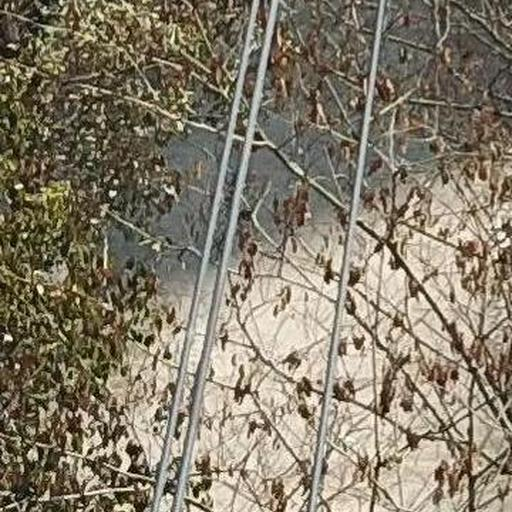
\includegraphics[width = 1.40in]{imgs/pldu_base_imgs/355.jpg}} &
  \subfloat{
\includegraphics[width = 1.40in]{imgs/pldu_gt/355.png}} &
  \subfloat{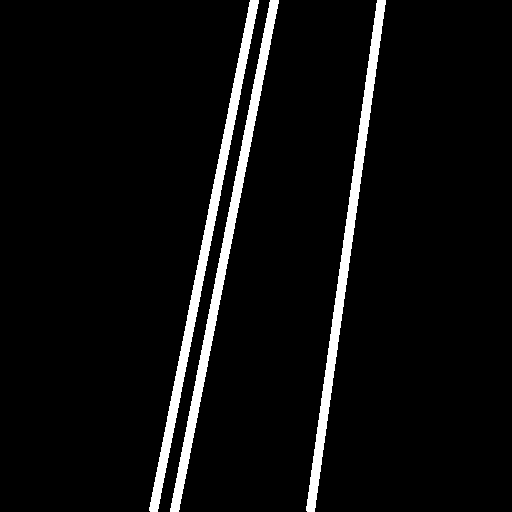
\includegraphics[width = 1.40in]{imgs/hawp/pldu_ha/355.png}} &
  \subfloat{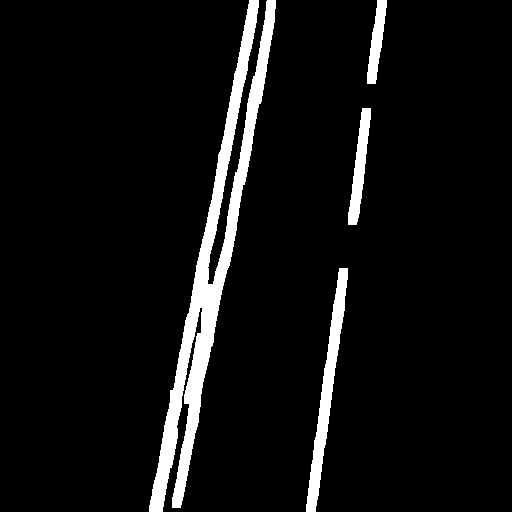
\includegraphics[width = 1.40in]{imgs/pldu_old/355.png}} &
  \subfloat{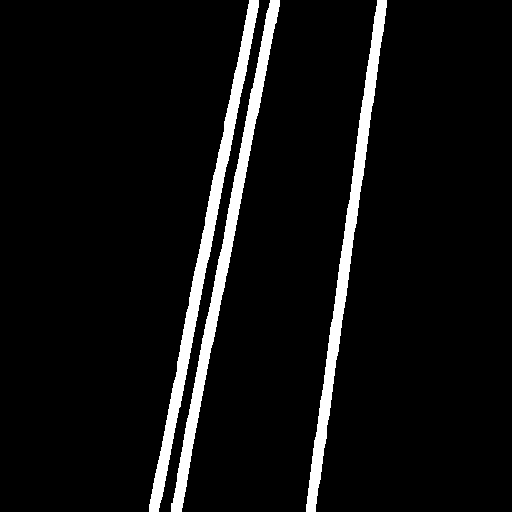
\includegraphics[width = 1.40in]{imgs/pldu_new/355.png}} \\
  \subfloat{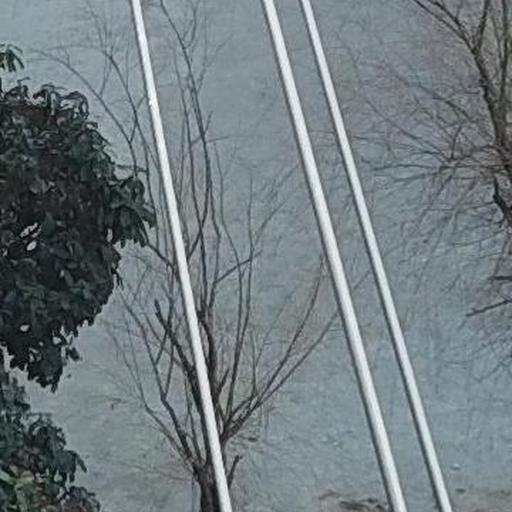
\includegraphics[width = 1.40in]{imgs/pldu_base_imgs/637.jpg}} &
  \subfloat{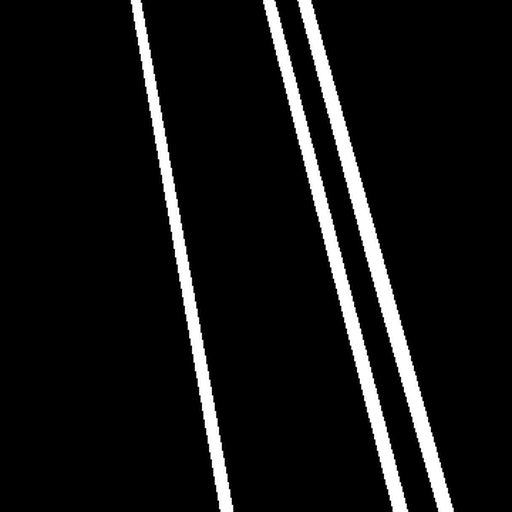
\includegraphics[width = 1.40in]{imgs/pldu_gt/637.png}} &
  \subfloat{
\includegraphics[width = 1.40in]{imgs/hawp/pldu_ha/637.png}} &
  \subfloat{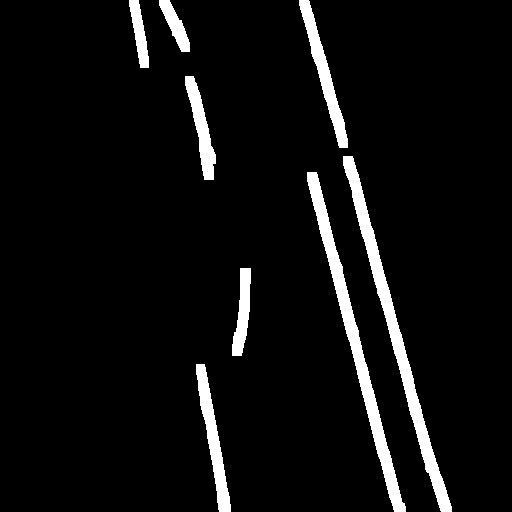
\includegraphics[width = 1.40in]{imgs/pldu_old/637.png}} &
  \subfloat{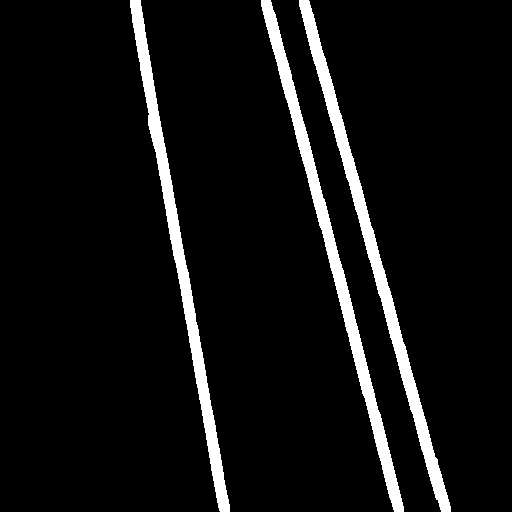
\includegraphics[width = 1.40in]{imgs/pldu_new/637.png}} \\
  \subfloat{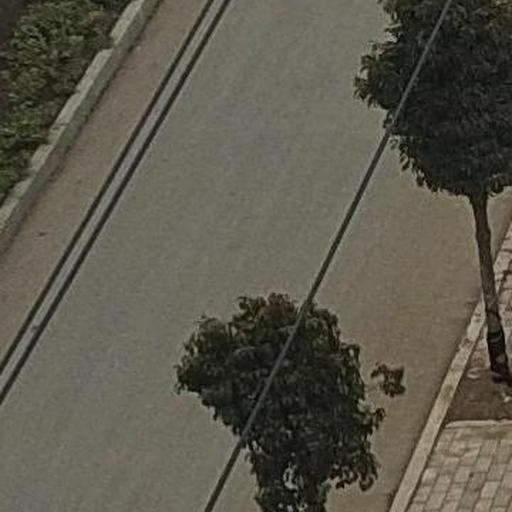
\includegraphics[width = 1.40in]{imgs/pldu_base_imgs/250.jpg}} &
  \subfloat{
\includegraphics[width = 1.40in]{imgs/pldu_gt/250.png}} &
  \subfloat{
\includegraphics[width = 1.40in]{imgs/hawp/pldu_ha/250.png}} &
  \subfloat{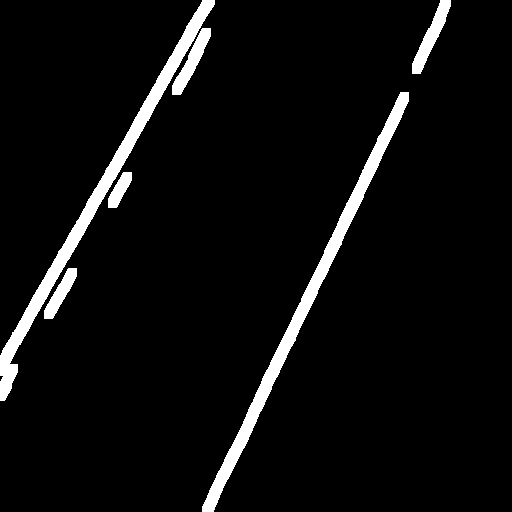
\includegraphics[width = 1.40in]{imgs/pldu_old/250.png}} &
  \subfloat{
\includegraphics[width = 1.40in]{imgs/pldu_new/250.png}} \\
  \subfloat{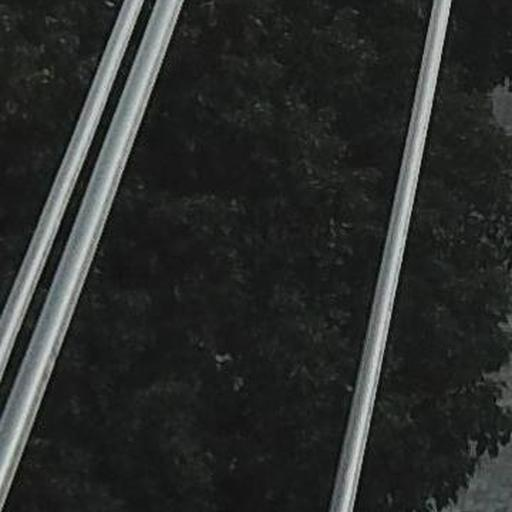
\includegraphics[width = 1.40in]{imgs/pldu_base_imgs/510.jpg}} &
  \subfloat{
\includegraphics[width = 1.40in]{imgs/pldu_gt/510.png}} &
  \subfloat{
\includegraphics[width = 1.40in]{imgs/hawp/pldu_ha/510.png}} &
  \subfloat{
\includegraphics[width = 1.40in]{imgs/pldu_old/510.png}} &
  \subfloat{
\includegraphics[width = 1.40in]{imgs/pldu_new/510.png}} \\
  \subfloat{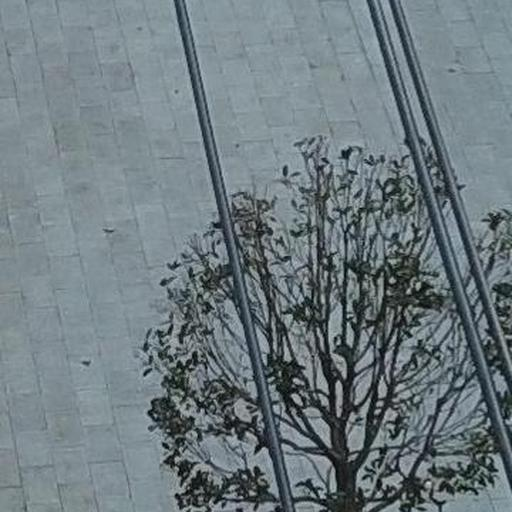
\includegraphics[width = 1.40in]{imgs/pldu_base_imgs/409.jpg}} &
  \subfloat{
\includegraphics[width = 1.40in]{imgs/pldu_gt/409.png}} &
  \subfloat{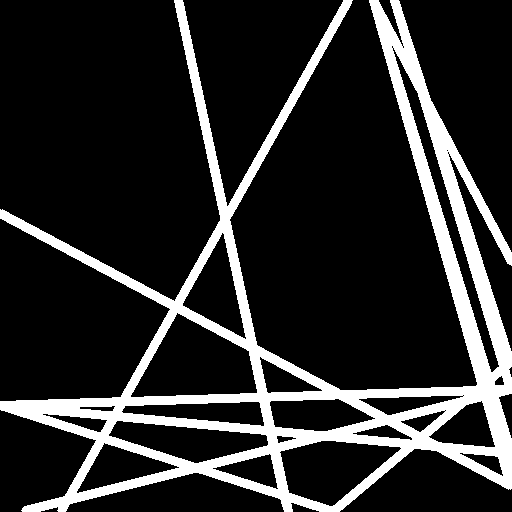
\includegraphics[width = 1.40in]{imgs/hawp/pldu_ha/409.png}} &
  \subfloat{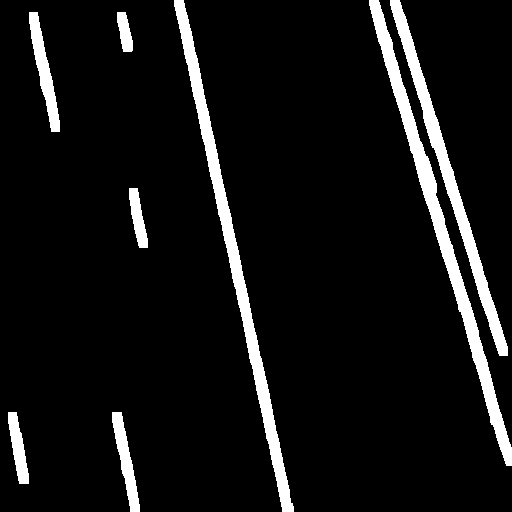
\includegraphics[width = 1.40in]{imgs/pldu_old/409.png}} &
  \subfloat{
\includegraphics[width = 1.40in]{imgs/pldu_new/409.png}} \\
  \subfloat{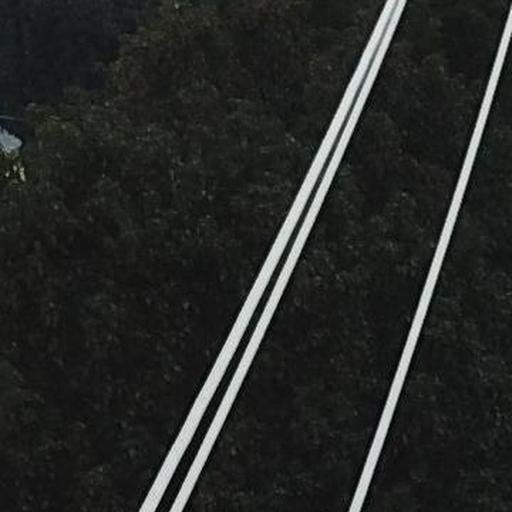
\includegraphics[width = 1.40in]{imgs/pldu_base_imgs/481.jpg}} &
  \subfloat{
\includegraphics[width = 1.40in]{imgs/pldu_gt/481.png}} &
  \subfloat{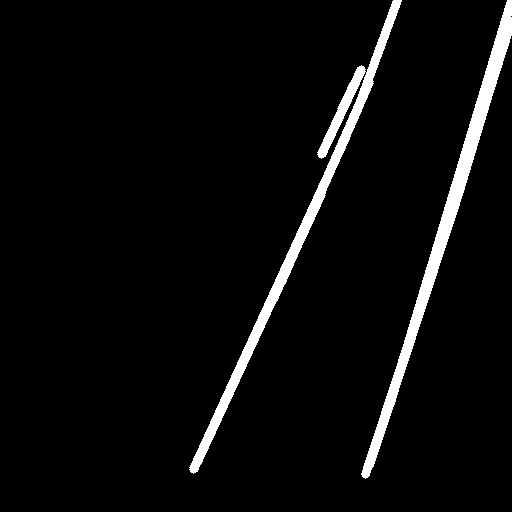
\includegraphics[width = 1.40in]{imgs/hawp/pldu_ha/481.png}} &
  \subfloat{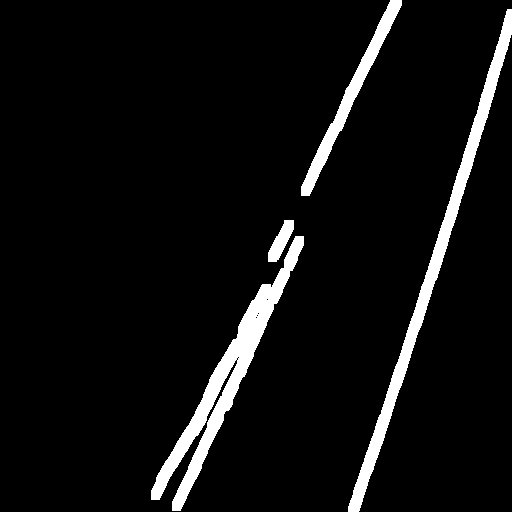
\includegraphics[width = 1.40in]{imgs/pldu_old/481.png}} &
  \subfloat{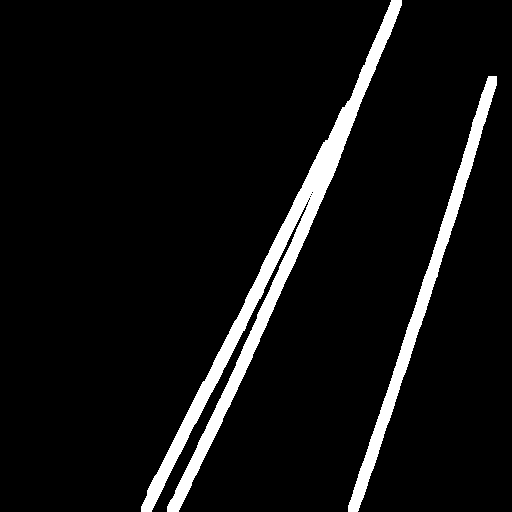
\includegraphics[width = 1.40in]{imgs/pldu_new/481.png}}\\
  % \subfloat{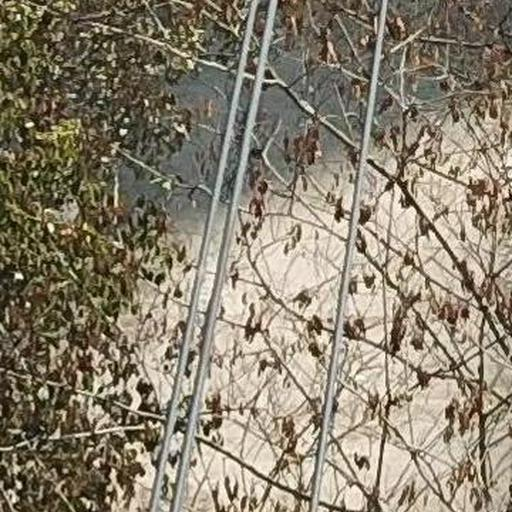
\includegraphics[width = 265in]{imgs/pldu_base_imgs/358.jpg}} &
  % \subfloat{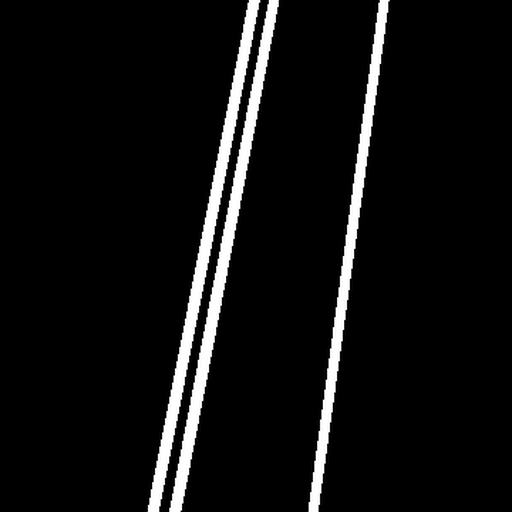
\includegraphics[width = 265in]{imgs/pldu_gt/358.png}} &
  % \subfloat{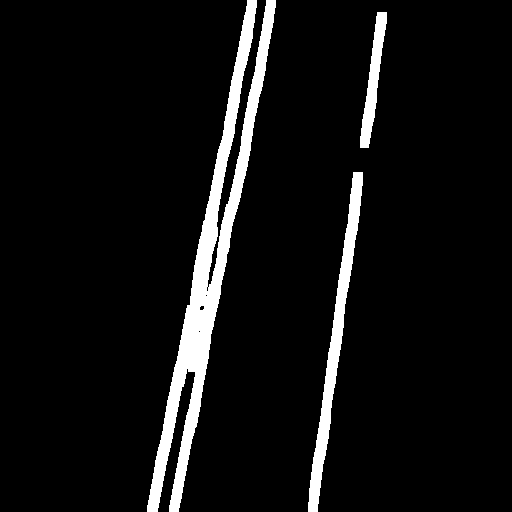
\includegraphics[width = 265in]{imgs/pldu_old/358.png}} &
  % \subfloat{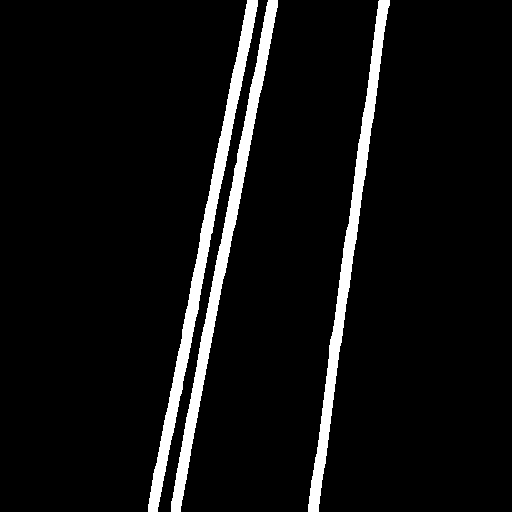
\includegraphics[width = 265in]{imgs/pldu_new/358.png}}\\
  

  % Add caption row
  Image & Ground truth & HAWPv2 & LSNet & LSNetv2
  % \subfloat[caption]{\includegraphics[width = 1.5in]{something}}\\
  \end{tabularx}
  \caption{\label{PLDU_example}Example test results of LSNet and LSNetv2 on test images in PLDU dataset. The columns from left to right contain: original images, ground truth segment map, outputs of HAWPv2, outputs of LSNet and outputs of LSNetv2}
\end{figure*}

\begin{figure*}
  \addtolength{\tabcolsep}{-5pt} 
  \begin{tabularx}{\textwidth}{ccccc}
  \centering
  \subfloat{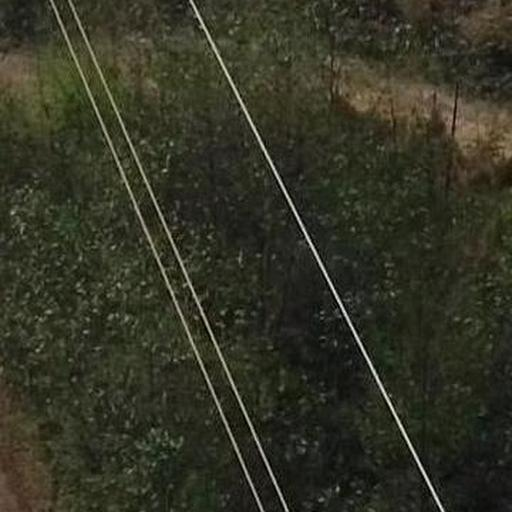
\includegraphics[width = 1.40in]{imgs/pldm_base_imgs/18.jpg}} &
  \subfloat{
\includegraphics[width = 1.40in]{imgs/pldm_gt/18.png}} &
  \subfloat{
\includegraphics[width = 1.40in]{imgs/hawp/pldm_ha/18.png}} &
  \subfloat{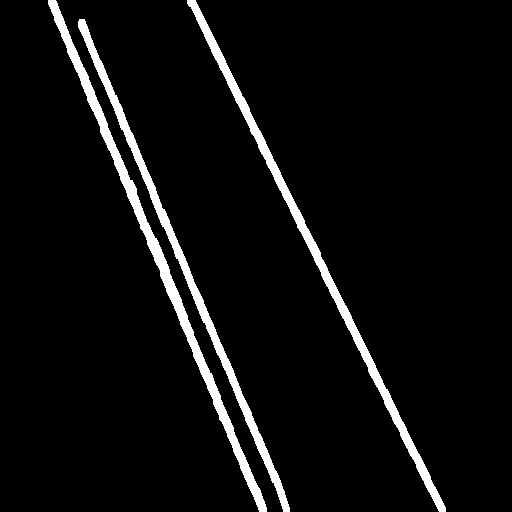
\includegraphics[width = 1.40in]{imgs/pldm_old/18.png}} &
  \subfloat{
\includegraphics[width = 1.40in]{imgs/pldm_new/18.png}} \\
  \subfloat{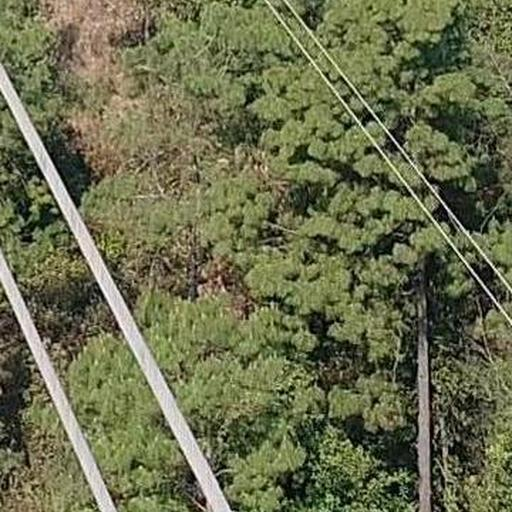
\includegraphics[width = 1.40in]{imgs/pldm_base_imgs/4.jpg}} &
  \subfloat{
\includegraphics[width = 1.40in]{imgs/pldm_gt/4.png}} &
  \subfloat{\includegraphics[width = 1.40in]{imgs/hawp/pldm_ha/4.png}} &
  \subfloat{\includegraphics[width = 1.40in]{imgs/pldm_old/4.png}} &
  \subfloat{\includegraphics[width = 1.40in]{imgs/pldm_new/4.png}} \\
  \subfloat{\includegraphics[width = 1.40in]{imgs/pldm_base_imgs/24.jpg}} &
  \subfloat{\includegraphics[width = 1.40in]{imgs/pldm_gt/24.png}} &
  \subfloat{\includegraphics[width = 1.40in]{imgs/hawp/pldm_ha/24.png}} &
  \subfloat{\includegraphics[width = 1.40in]{imgs/pldm_old/24.png}} &
  \subfloat{\includegraphics[width = 1.40in]{imgs/pldm_new/24.png}} \\
  \subfloat{\includegraphics[width = 1.40in]{imgs/pldm_base_imgs/124.jpg}} &
  \subfloat{\includegraphics[width = 1.40in]{imgs/pldm_gt/124.png}} &
  \subfloat{\includegraphics[width = 1.40in]{imgs/hawp/pldm_ha/124.png}} &
  \subfloat{\includegraphics[width = 1.40in]{imgs/pldm_old/124.png}} &
  \subfloat{\includegraphics[width = 1.40in]{imgs/pldm_new/124.png}} \\

  % Add caption row
  Image & Ground truth & HAWPv2 & LSNet & LSNetv2
  % \subfloat[caption]{\includegraphics[width = 1.5in]{something}}\\
  \end{tabularx}
  \caption{\label{PLDM_example}Example test results of LSNet and LSNetv2 on test images in PLDM dataset. The columns from left to right contain: original images, ground truth segment map, outputs of HAWPv2, outputs of LSNet and outputs of LSNetv2}
\end{figure*}

 Results in Table~\ref{res1_table} illustrate that LSNetv2 consistently outperforms LSNet across all datasets considered. The difference is most pronounced when considering the APR metric, leading to a performance improvement when considering the $F_{\beta}$ metric. The performance gap is largest for the TTPLA and Esmart datasets, which can be attributed to them being arguably more complex datasets.  From Fig \ref{ttpla_example_0}, we can see that the TTPLA dataset contains many images with several semi-parallel powerlines in close proximity to each other, which showcases the effectiveness of LSNetv2 to a larger degree leading to the biggest performance gap among the four datasets. LSNetv2 is able to both detect more true positive line segments and semantic powerlines. In the Esmart dataset, as aforementioned, due to the need to also detect guy wires, each image in this dataset usually contains at least one visual crossing. As shown in Fig \ref{esmart_example_0}, unlike LSNetv2, LSNet, by design, can not detect the two line segments at the crossings. Further, it can be observed that LSNetv2 is even better than LSNet in general one-line-segment-per-cell cases, especially when the visibility of the line segments is limited due to camera angle and distance, which make the line segments thin, and/or background blending. This can partially be attributed to the ConvNext backbone by providing filters with a larger receptive field that, together with other modernized features, allows LSNetv2 to get global information across the images to make accurate inferences at each cell.
 
 The performance gap is smaller for the PLDU and PLDM datasets since these datasets are subjectively less difficult than the other two. Similarly to the two previous cases, the improvement lies mainly in the APR metric. There are no explicit line crossings found in the test set and in cases where there are parallel powerlines in close proximity, the four-grid design of LSNet may help compensate for when a line segment is not detected by one of the four grids. However, as shown in Fig \ref{PLDU_example}-\ref{PLDM_example}, the missing line segment problem still exists for LSNet leading to the eventual miss-detection of the whole powerline. Furthermore, close line segments may confuse LSNet resulting in imprecise localization of endpoints implied by the occasional fillings in the gaps between powerlines, such as the examples shown in the first column of Fig \ref{PLDU_example}. This might cause further complications for potential downstream instance segmentation tasks. LSNetv2 is more robust to such close-proximity cases and can produce output masks with fewer missing segments and with clearer and more precise division between powerlines. The last row of Fig \ref{PLDU_example} shows that LSNet is susceptible to confusion by background lines, while LSNetv2 appears to be more resistant. This can be attributed to ConvNext being able to mimic the non-local self-attention mechanism of the Vision Transformer \cite{vit}, which helps gather more global information, helping LSNetv2 to better differentiate between semantic line segments.



Table \ref{res1_table} further shows the quantitative results of HAWPv2. Note, we observed that the performance of HAWPv2, estimated by either $F_1$ or $F_\beta$, was heavily dependent on different choices of line width and the score threshold (used to filter out unconfident line segments). Thus, for HAWPv2, we considered two settings, the one that leads to the best $F_1$ score and the one yielding the best $F_\beta$ score. Table \ref{hawp_prop} shows the configuration choices, at which these highest metric values were achieved for each dataset. Overall, the best values are achieved at line widths similar to those used when calculating the metrics for LSNet and LSNetv2. In addition, high score thresholds lead to higher APR and $F_\beta$ at the expense of ARR and vice versa, which is expected. Overall, LSNetv2 is able to outperform the best $F_1$ score and $F_\beta$ score across all datasets. Fig \ref{PLDU_example} - \ref{esmart_example_0} show that HAWPv2 is able to detect entire powerlines consistently, however, false positive and false negative regions are often larger than those observed in LSNetv2. This can be attributed to the 4-overlapping-grid design, where missing line segments in each cell can be compensated by its neighbors and, since each cell is only responsible for a small region, false positives occuring in one cell do not have a significant impact. Another interesting insight is that HAWPv2 has higher performance than LSNet for the TTPLA and Esmart datasets while the reverse is true for the PLDU and PLDM datasets. This makes sense since HAWPv2 does not have the limitations of being only able to detect one line segment per cell and, thus, is more competitive on the TTPA and Esmart datasets.


\subsection{Ablation Study}
We conduct ablation experiments on the TTPLA and Esmart datasets and present results in Table \ref{ablation_ttpla} and \ref{ablation_esmart}, respectively. We can see the following overall trend for both datasets: removing any of the three proposed components of LSNetv2 results in a degradation in terms of $F_{\beta}$ score, highlighting their importance to the overall model. Further, we note that adding any of the components to the original LSNet (top row), improves the LSNet performance.
%the increasing addition of the three components provide LSNetv2 with increasingly better performance, most obviously in terms of $F_{\beta}$ score. Specifically, the addition of either of the components is more beneficial than none and the addition of a pair among the three components often produce superior metric values than only individual components. 
Finally, the combination of the three achieve the most desirable performance, providing considerable boost in both  $F_1$ and $F_{\beta}$ score.

For the Esmart dataset, ConvNext is clearly a beneficial addition which gives LSNetv2 improvements in both $F_1$ and $F_{\beta}$ scores. The benefits are also noticable when concerning the addition of the multi-guess capability brought about by bipartite matching and the ordered loss. These two components individually improved $F_{\beta}$ score while maintaining comparable $F_1$ score. Combining the ConvNext-Tiny backbone with either the multi-guess capability or the ordered loss, instead, achieves a noticable performance increase when compared to just using the multi-guess capability or the ordered loss alone. This further validates the benefit of having ConvNext-Tiny with its increased receptive field as the new backbone. 
For the TTPLA dataset, we observe that the addition of each of the components individually provides noticeable improvements in $F_1$ and $F_{\beta}$ score. 
In particular, the addition of the ConvNext-Tiny backbone provides a significant performance boost indicated in the jumps in both $F_1$ and $F_{\beta}$ score. Pairings ConvNext-Tiny with one of the other contributions, provides models with higher APR and $F_{\beta}$ but with lowered ARR and $F_1$ when compared to just ConvNext-Tiny alone. This is acceptable since the $F_{\beta}$ metric is more preferable as explained in \ref{evaluation_metrics} and the ARR values are still comparable to the base case where no components are addded. In addition, this is understandable since the bipartite matching task provides LSNetv2 with the ability to detect multi-line-segments per cell but might pose a harder challenge for the model to train. Also, the ordered loss is observed to be particularly relevant when paired with the harder training task brought about by bipartite matching. In fact, for both datasets, the combinations of bipartite matching and ordered loss generated models with better performance than if the two components are used alone. 
%Finally, it can be seen that the inclusion of all the components provides the best overall performance.

\subsection{Backbone Analysis}

To further validate the benefit of the ConvNext-Tiny backbone, we compare ConvNext-Tiny with the original modified VGG-16 architecture, as well as a Resnet-50 and Efficientnetv2-M backbone. The detailed architecture is shown in table \ref{backbone_arch}.

Table \ref{backbone_res_table} shows the results of our experimentation with other backbones. Overall, the ConvNext-Tiny backbone is superior to the other alternatives, helping LSNetv2 reach the highest $F_1$ and $F_\beta$ scores across almost all scenarios. In addition with ConvNext-Tiny being in one of the state-of-the-art families of CNNs, the performance of this backbone can be attributed to it having the biggest theoretical receptive field, more than double the size of the input image. This means that each cell inference produced by this network can hypothetically gain information from the entire image.  LSNetv2 with the modified VGG-16 backbone has competitive performance versus the first version of LSNet for all datasets except for PLDM, where LSNetv2 has a comparable $F_1$ score but noticeably lower APR and $F_{\beta}$ score. This can be attributed to the limited need for multi-line-segment-per-cell detection when considering the PLDU and PLDM datasets. Additionally, in these scenarios, the introduction of bipartite matching might result in more challenging optimization due to the additional degree of freedom when training LSNetv2. %built on the modified-VGG. 
Nevertheless, for the more challenging TTPLA and Esmart datasets, which benefit from the multi-line-segment detection capability, LSNetv2 with modified-VGG backbone achieves considerably better performance than the original LSNet. LSNetv2 with Resnet-50 backbone is consistently the second-best across all cases despite having a relatively smaller theoretical receptive field and the lowest number of trainable parameters. This is expected since Resnet, as well as ConvNext, are equipped with skip connections, which have been demonstrated to smoothen the optimization landscape \cite{li2018visualizing}. The VGG on the other hand, does not make use of these, making it harder to optimize. Efficientnetv2-M is another relatively recent architecture that is competitive at image classification \cite{efficientnetv2} and object detection \cite{efficientdet}. It also has a high theoretical receptive field (technically covers the entire image due to the squeeze-and-excitation blocks), as well as skip connections. However, this backbone is consistently inferior than the rest, including the original modified-VGG backbone. This might be because EfficientnetV2 was designed specifically to achieve high accuracy for image classification and, even though this architecture family also performs well for object detection and semantic segmentation \cite{efficientnetv2}, EfficientnetV2 is simply not suitable for the tasks of LSNetv2. Also, since EfficientnetV2 was designed with high level of specificity via a compound scaling method, thus, any modification, such as truncation in this case, can have a higher negative effect to the performance.%This, together with ConvNext-Tiny being built upon the ResNet family, might suggest that the ResNet design is a good fit for the backbone of LSNetv2, and from our experiments, ConvNext-Tiny is currently the best candidate.




% \begin{table*}[]
% \begin{tabular}{lllll|llll|llll|llll}
%         & \multicolumn{4}{c|}{PLDU}           & \multicolumn{4}{c|}{PLDM}           & \multicolumn{4}{c|}{TTPLA}          & \multicolumn{4}{c}{Esmart}          \\ \cline{2-17} 
%         & APR   & ARR   & $F_1$ & $F_{\beta}$ & APR   & ARR   & $F_1$ & $F_{\beta}$ & APR   & ARR   & $F_1$ & $F_{\beta}$ & APR   & ARR   & $F_1$ & $F_{\beta}$ \\ \hline
% HAWP (best $F_1$)       & 0.830 & 0.649 & 0.728 & 0.812       & 0.815 & 0.664 & 0.732 & 0.800       & 0.559 & 0.639 & 0.596 & 0.565       & 0.751 & 0.850 & 0.797 & 0.758       \\
% HAWP (best $F_\beta$)   & 0.939 & 0.532 & 0.679 & 0.883       & 0.953 & 0.448 & 0.610 & 0.872       & 0.650 & 0.324 & 0.432 & 0.600       & 0.805 & 0.680 & 0.737 & 0.793       \\
% LSNet                   & 0.914 & 0.662 & 0.767 & 0.886       & 0.916 & 0.726 & 0.810 & 0.896       & 0.579 & 0.525 & 0.551 & 0.574       & 0.726 & 0.812 & 0.766 & 0.732       \\
% LSNetv2                 & 0.938 & 0.666 & 0.779 & 0.907       & 0.934 & 0.724 & 0.815 & 0.912       & 0.714 & 0.560 & 0.628 & 0.698       & 0.845 & 0.814 & 0.829 & 0.842      
% \end{tabular}
% \caption{\label{res1_table} Result 1}
% \end{table*}




% \begin{table*}[]
% \begin{tabular}{lllll|llll|llll|llll}
%                  & \multicolumn{4}{c|}{PLDU}           & \multicolumn{4}{c|}{PLDM}           & \multicolumn{4}{c|}{TTPLA}          & \multicolumn{4}{c}{Esmart}          \\ \cline{2-17} 
% Backbone         & APR   & ARR   & $F_1$ & $F_{\beta}$ & APR   & ARR   & $F_1$ & $F_{\beta}$ & APR   & ARR   & $F_1$ & $F_{\beta}$ & APR   & ARR   & $F_1$ & $F_{\beta}$ \\ \hline
% modified VGG     & 0.899 & 0.685 & 0.778 & 0.876       & 0.818 & 0.793 & 0.805 & 0.815       & 0.696 & 0.566 & 0.624 & 0.683       & 0.759 & 0.813 & 0.785 & 0.763       \\
% Resnet-50        & 0.920 & 0.673 & 0.778 & 0.892       & 0.918 & 0.731 & 0.814 & 0.899       & 0.643 & 0.635 & 0.639 & 0.642       & 0.794 & 0.809 & 0.802 & 0.795       \\
% Efficientnetv2-M & 0.907 & 0.645 & 0.754 & 0.877       & 0.923 & 0.674 & 0.779 & 0.895       & 0.573 & 0.355 & 0.438 & 0.545       & 0.747 & 0.796 & 0.771 & 0.750       \\
% ConvNext-Tiny    & 0.938 & 0.666 & 0.779 & 0.907       & 0.934 & 0.724 & 0.815 & 0.912       & 0.714 & 0.560 & 0.628 & 0.698       & 0.845 & 0.814 & 0.829 & 0.842      
% \end{tabular}
% \caption{\label{backbone_res_table} Backbone analysis}
% \end{table*}

\newcommand\vggone{
    $3 \times 3, 64$ \\
    $3 \times 3, 64$ \\
    $1 \times 3, 64, \text{, s=2}$ \\
}

\newcommand\vggtwo{
    $3 \times 3, 128$ \\
    $3 \times 3, 128$ \\
    $1 \times 3, 128, \text{, s=2}$ \\
}
\newcommand\vggthree{
    $3 \times 3, 256$ \\
    $3 \times 3, 256$ \\
    $1 \times 3, 256, \text{, s=2}$ \\
}
\newcommand\vggfour{
    $3 \times 3, 512$ \\
    $3 \times 3, 512$ \\
    $1 \times 3, 512, \text{, s=2}$ \\
}

\newcommand\branch{
    $2 \times 2, 512$ \\
    $1 \times 1, \text{2 * 10 or 4 * 10}$ \\
}
%%%%%%%%%%%%%%%%%%%%%%%%%%%%%%%%%%%%%%%%
\newcommand\resone{
    7 \times 7 \text{, s=2 } \\
}



\newcommand\restwo{
    3 \times 3 \text{ maxpool, s=2 } \\
    \schema{
    \schemabox{$3 \times$}
    }
    {
    \schemabox{
    $1 \times 1, 64$ \\
    $3 \times 3, 64$ \\
    $1 \times 3, 256$ \\
    }
    }
}

\newcommand\resthree{
    \schema{
    \schemabox{$1 \times$}
    }
    {
    \schemabox{
    $1 \times 1, 128 \text{, s=2}$ \\
    $3 \times 3, 128$ \\
    $1 \times 3, 512$ \\
    }
    }\\
    \schema{
    \schemabox{$3 \times$}
    }
    {
    \schemabox{
    $1 \times 1, 128$ \\
    $3 \times 3, 128$ \\
    $1 \times 3, 512$ \\
    }
    }
}

\newcommand\resfour{
    \schema{
    \schemabox{$1 \times$}
    }
    {
    \schemabox{
    $1 \times 1, 256 \text{, s=2}$ \\
    $3 \times 3, 256$ \\
    $1 \times 3, 1024$ \\
    }
    }\\
    \schema{
    \schemabox{$5 \times$}
    }
    {
    \schemabox{
    $1 \times 1, 256$ \\
    $3 \times 3, 256$ \\
    $1 \times 3, 1024$ \\
    }
    }
}
%%%%%%%%%%%%%%%%%%%%%%%%%%%%%%%%%%%%%%%%%%%%%%%%%%%
\newcommand\effone{
    3 \times 3, 24 \text{, s=2 } \\
    \schema{
    \schemabox{$3 \times$}
    }
    {
    \schemabox{
    $3 \times 3, 24$\\
    }
    } \\
}
\newcommand\efftwo{
$3 \times 3, 96 \text{, s=2}$\\
$1 \times 1, 48$ \\
\schema{
    
    \schemabox{$4 \times$}
    }
    {
    \schemabox{
    $3 \times 3, 192$\\
    $1 \times 1, 48$
    }
    } \\
}

\newcommand\effthree{
$3 \times 3, 192 \text{, s=2}$\\
$1 \times 1, 80$ \\
\schema{
    
    \schemabox{$4 \times$}
    }
    {
    \schemabox{
    $3 \times 3, 320$\\
    $1 \times 1, 80$
    }
    } \\
}

\newcommand\efffour{
$1 \times 1, 320$ \\
$\text{dw } 3 \times 3, 320, s=2$\\
SE-Block(ratio=0.25) \\
$1 \times 1, 160$ \\
 \schema{
\schemabox{$6 \times$}
}
{
\schemabox{
$1 \times 1, 640$ \\
$\text{dw } 3 \times 3, 640$\\
SE-Block(ratio=0.25) \\
$1 \times 1, 160$ \\
}
} \\
}

\newcommand\efffive{
$1 \times 1, 960$ \\
$\text{dw } 3 \times 3, 960$\\
SE-Block(ratio=0.25) \\
$1 \times 1, 176$ \\
 \schema{
\schemabox{$13 \times$}
}
{
\schemabox{
$1 \times 1, 1056$ \\
$\text{dw } 3 \times 3, 1056$\\
SE-Block(ratio=0.25) \\
$1 \times 1, 176$ \\
}
} \\
$1 \times 1, 1056$ \\
}
%%%%%%%%%%%%%%%%%%%%%%%%%%%%%%%%%%%%%%%%%%%%%%%%%%%
\newcommand\convnextone{
    4 \times 4, 96 \text{, s=4 } \\
}

\newcommand\convnexttwo{
    \schema{
    \schemabox{$3 \times$}
    }
    {
    \schemabox{
    $7 \times 7, 96$\\
    $1 \times 1, 384$ \\
    $1 \times 1, 96$ \\
    }
    } \\
    2 \times 2, 192, \text{ s=2}
    
}

\newcommand\convnextthree{
    \schema{
    \schemabox{$3 \times$}
    }
    {
    \schemabox{
    dw $7 \times 7, 192$\\
    $1 \times 1, 768$ \\
    $1 \times 1, 192$ \\
    }
    } \\
    2 \times 2, 384, \text{ s=2}
    
}

\newcommand\convnextfour{
    \schema{
    \schemabox{$9 \times$}
    }
    {
    \schemabox{
    dw $7 \times 7, 384$\\
    $1 \times 1, 1536$ \\
    $1 \times 1, 384$ \\
    }
    }
}

\begin{table*}[]
\centering
\begin{tabular}{l|l|l|l|l|l}
Stage & Output size & Modified VGG & Resnet-50 & EfficientnetV2-M & ConvNext-Tiny \\ \hline
1     & $256 \times 256$   & \makecell{\vggone}      & \makecell{\resone}    & \makecell{\effone} &               \\ \hline
2     & $128 \times 128$   & \makecell{\vggtwo}      & \makecell{\restwo}  & \makecell{\efftwo}  & \makecell{\convnextone} \\ \hline
3     & $64 \times 64$     & \makecell{\vggthree}    & \makecell{\resthree}          & \makecell{\effthree} & \makecell{\convnexttwo}   \\ \hline
4     & $32 \times 32$     & \makecell{\vggfour}     & \makecell{\resfour}          & \makecell{\efffour}  & \makecell{\convnextthree}  \\ \hline
5     & $32 \times 32$     &              &           & \makecell{\efffive}  & \makecell{\convnextfour}   \\ \hline
\pbox{20cm}{Classifier or \\ Regressor module} & $31 \times 31$     & \multicolumn{4}{c}{\makecell{\branch}}                 \\ \hline
Receptive field     &              & 91         & 291          & 779 (inf)           & 1096                 \\ \hline
Parameters (M)      &              & 10.0       & 12.8          & 14.5           & 13.9 
\end{tabular}
\caption{\label{backbone_arch} Architecture of LSNetv2 using different CNNs as backbone. \textit{$ a \times a, b, \text{s}=c$} indicates a convolutional layer with kernel size $a$, number of filters $b$ and stride $c$. \textit{dw} indicates a depthwise convolutional layer. The curl brackets signals groups of layers with skip connections. This table excludes information about the skip connections, normalization and activation layers.}
\end{table*}

\begin{table*}[]
\caption{\label{backbone_res_table} Performance of LSNetv2 using different CNNs as backbone.}
\resizebox{\textwidth}{!}{
\begin{tabular}{lllll|llll|llll|llll}
                 & \multicolumn{4}{c|}{PLDU}           & \multicolumn{4}{c|}{PLDM}           & \multicolumn{4}{c|}{TTPLA}          & \multicolumn{4}{c}{Esmart}          \\ \cline{2-17} 
Backbone         & APR   & ARR   & $F_1$ & $F_{\beta}$ & APR   & ARR   & $F_1$ & $F_{\beta}$ & APR   & ARR   & $F_1$ & $F_{\beta}$ & APR   & ARR   & $F_1$ & $F_{\beta}$ \\ \hline
modified VGG     & 0.899 & 0.685 & 0.778 & 0.838       & 0.818 & 0.793 & 0.805 & 0.812       & 0.696 & 0.566 & 0.624 & 0.660       & 0.759 & 0.813 & 0.785 & 0.770       \\
Resnet-50        & 0.920 & 0.673 & 0.778 & 0.848       & 0.918 & 0.731 & 0.814 & 0.866       & 0.643 & 0.635 & 0.639 & 0.641       & 0.794 & 0.809 & 0.802 & 0.797       \\
Efficientnetv2-M & 0.907 & 0.645 & 0.754 & 0.829       & 0.923 & 0.674 & 0.779 & 0.850       & 0.573 & 0.355 & 0.438 & 0.501       & 0.747 & 0.796 & 0.771 & 0.757       \\
ConvNext-Tiny    & 0.938 & 0.666 & 0.779 & 0.857       & 0.934 & 0.724 & 0.815 & 0.875       & 0.714 & 0.560 & 0.628 & 0.671       & 0.845 & 0.814 & 0.829 & 0.837      
\end{tabular}}
\end{table*}





\begin{figure*}
  \addtolength{\tabcolsep}{-5pt} 
  \begin{tabularx}{\textwidth}{ccccc}
  \centering
  \subfloat{\includegraphics[width = 1.40in]{imgs/ttpla_base_imgs/107_1410_2.jpg}} &
  \subfloat{\includegraphics[width = 1.40in]{imgs/ttpla_gt/107_1410_2.png}} &
  \subfloat{\includegraphics[width = 1.40in]{imgs/hawp/ttpla_ha/107_1410_2.png}} &
  \subfloat{\includegraphics[width = 1.40in]{imgs/ttpla_old/107_1410_2.png}} &
  \subfloat{\includegraphics[width = 1.40in]{imgs/ttpla_new/107_1410_2.png}} \\
  \subfloat{\includegraphics[width = 1.40in]{imgs/ttpla_base_imgs/25_00272_1.jpg}} &
  \subfloat{\includegraphics[width = 1.40in]{imgs/ttpla_gt/25_00272_1.png}} &
  \subfloat{\includegraphics[width = 1.40in]{imgs/hawp/ttpla_ha/25_00272_1.png}} &
  \subfloat{\includegraphics[width = 1.40in]{imgs/ttpla_old/25_00272_1.png}} &
  \subfloat{\includegraphics[width = 1.40in]{imgs/ttpla_new/25_00272_1.png}} \\
  % \subfloat{\includegraphics[width = 1.40in]{imgs/ttpla_base_imgs/14_00486_2.jpg}} &
  % \subfloat{\includegraphics[width = 1.40in]{imgs/ttpla_gt/14_00486_2.png}} &
  % \subfloat{\includegraphics[width = 1.40in]{imgs/hawp/ttpla_ha/14_00486_2.png}} &
  % \subfloat{\includegraphics[width = 1.40in]{imgs/ttpla_old/14_00486_2.png}} &
  % \subfloat{\includegraphics[width = 1.40in]{imgs/ttpla_new/14_00486_2.png}} \\
  \subfloat{\includegraphics[width = 1.40in]{imgs/ttpla_base_imgs/23_00706_2.jpg}}&
  \subfloat{\includegraphics[width = 1.40in]{imgs/ttpla_gt/23_00706_2.png}}&
  \subfloat{\includegraphics[width = 1.40in]{imgs/hawp/ttpla_ha/23_00706_2.png}}&
  \subfloat{\includegraphics[width = 1.40in]{imgs/ttpla_old/23_00706_2.png}}&
  \subfloat{\includegraphics[width = 1.40in]{imgs/ttpla_new/23_00706_2.png}}\\

  \subfloat{\includegraphics[width = 1.40in]{imgs/ttpla_base_imgs/110_0_1.jpg}}&
  \subfloat{\includegraphics[width = 1.40in]{imgs/ttpla_gt/110_0_1.png}}&
  \subfloat{\includegraphics[width = 1.40in]{imgs/hawp/ttpla_ha/110_0_1.png}}&
  \subfloat{\includegraphics[width = 1.40in]{imgs/ttpla_old/110_0_1.png}}&
  \subfloat{\includegraphics[width = 1.40in]{imgs/ttpla_new/110_0_1.png}}\\
  \subfloat{\includegraphics[width = 1.40in]{imgs/ttpla_base_imgs/25_00667_2.jpg}}&
  \subfloat{\includegraphics[width = 1.40in]{imgs/ttpla_gt/25_00667_2.png}}&
  \subfloat{\includegraphics[width = 1.40in]{imgs/hawp/ttpla_ha/25_00667_2.png}}&
  \subfloat{\includegraphics[width = 1.40in]{imgs/ttpla_old/25_00667_2.png}}&
  \subfloat{\includegraphics[width = 1.40in]{imgs/ttpla_new/25_00667_2.png}}\\
  \subfloat{\includegraphics[width = 1.40in]{imgs/ttpla_base_imgs/42_00551_1.jpg}}&
  \subfloat{\includegraphics[width = 1.40in]{imgs/ttpla_gt/42_00551_1.png}}&
  \subfloat{\includegraphics[width = 1.40in]{imgs/hawp/ttpla_ha/42_00551_1.png}}&
  \subfloat{\includegraphics[width = 1.40in]{imgs/ttpla_old/42_00551_1.png}}&
  \subfloat{\includegraphics[width = 1.40in]{imgs/ttpla_new/42_00551_1.png}}\\
  
  % \subfloat{\includegraphics[width = 1.65in]{imgs/ttpla_base_imgs/25_00272_1.jpg}} &
  % \subfloat{\includegraphics[width = 1.65in]{imgs/ttpla_gt/25_00272_1.png}} &
  % \subfloat{\includegraphics[width = 1.65in]{imgs/ttpla_old/25_00272_1.png}} &
  % \subfloat{\includegraphics[width = 1.65in]{imgs/ttpla_new/25_00272_1.png}}\\

  % Add caption row
  Image & Ground truth & HAWPv2 & LSNet & LSNetv2
  % \subfloat[caption]{\includegraphics[width = 1.5in]{something}}\\
  \end{tabularx}
  \caption{\label{ttpla_example_0}Example test results of LSNet and LSNetv2 on test images in PLDU dataset. The columns from left to right contain: original images, ground truth segment map, outputs of HAWPv2, outputs of LSNet and outputs of LSNetv2}
\end{figure*}

% \begin{figure*}
%   \begin{tabularx}{\textwidth}{cccc}
%   \centering
%   \subfloat{\includegraphics[width = 1.65in]{imgs/ttpla_base_imgs/25_00667_2.jpg}} &
%   \subfloat{\includegraphics[width = 1.65in]{imgs/ttpla_base_imgs/33_7545_1.jpg}} &
%   \subfloat{\includegraphics[width = 1.65in]{imgs/ttpla_base_imgs/42_00551_1.jpg}} &
%   \subfloat{\includegraphics[width = 1.65in]{imgs/ttpla_base_imgs/47_00101_1.jpg}}\\
%   \subfloat{\includegraphics[width = 1.65in]{imgs/ttpla_gt/25_00667_2.png}} &
%   \subfloat{\includegraphics[width = 1.65in]{imgs/ttpla_gt/33_7545_1.png}} &
%   \subfloat{\includegraphics[width = 1.65in]{imgs/ttpla_gt/42_00551_1.png}} &
%   \subfloat{\includegraphics[width = 1.65in]{imgs/ttpla_gt/47_00101_1.png}}\\
%   \subfloat{\includegraphics[width = 1.65in]{imgs/hawp/ttpla_ha/25_00667_2.png}} &
%   \subfloat{\includegraphics[width = 1.65in]{imgs/hawp/ttpla_ha/33_7545_1.png}} &
%   \subfloat{\includegraphics[width = 1.65in]{imgs/hawp/ttpla_ha/42_00551_1.png}} &
%   \subfloat{\includegraphics[width = 1.65in]{imgs/hawp/ttpla_ha/47_00101_1.png}}\\
%   \subfloat{\includegraphics[width = 1.65in]{imgs/ttpla_old/25_00667_2.png}} &
%   \subfloat{\includegraphics[width = 1.65in]{imgs/ttpla_old/33_7545_1.png}} &
%   \subfloat{\includegraphics[width = 1.65in]{imgs/ttpla_old/42_00551_1.png}} &
%   \subfloat{\includegraphics[width = 1.65in]{imgs/ttpla_old/47_00101_1.png}}\\
%   \subfloat{\includegraphics[width = 1.65in]{imgs/ttpla_new/25_00667_2.png}} &
%   \subfloat{\includegraphics[width = 1.65in]{imgs/ttpla_new/33_7545_1.png}} &
%   \subfloat{\includegraphics[width = 1.65in]{imgs/ttpla_new/42_00551_1.png}} &
%   \subfloat{\includegraphics[width = 1.65in]{imgs/ttpla_new/47_00101_1.png}}\\
%   % \subfloat{\includegraphics[width = 1.65in]{imgs/ttpla_base_imgs/57_00141_2.jpg}} &
%   % \subfloat{\includegraphics[width = 1.65in]{imgs/ttpla_gt/57_00141_2.png}} &
%   % \subfloat{\includegraphics[width = 1.65in]{imgs/ttpla_old/57_00141_2.png}} &
%   % \subfloat{\includegraphics[width = 1.65in]{imgs/ttpla_new/57_00141_2.png}}\\
%   % \subfloat[caption]{\includegraphics[width = 1.5in]{something}}\\
%   \end{tabularx}
%   \caption{\label{ttpla_example_1}Second five example test results of LSNet and LSNetv2 on test images in PLDU dataset. The columns from left to right contain: original images, ground truth segment map, outputs of LSNet and outputs of LSNetv2}
% \end{figure*}

% \begin{figure*}
%   \begin{tabularx}{\textwidth}{ccccc}
%   \centering
%   \subfloat{\includegraphics[width = 1.65in]{imgs/ttpla_base_imgs/110_0_1.jpg}} &
%   \subfloat{\includegraphics[width = 1.65in]{imgs/ttpla_base_imgs/57_00141_2.jpg}}\\
%   \subfloat{\includegraphics[width = 1.65in]{imgs/ttpla_gt/110_0_1.png}} &
%   \subfloat{\includegraphics[width = 1.65in]{imgs/ttpla_gt/57_00141_2.png}}\\
%   \subfloat{\includegraphics[width = 1.65in]{imgs/hawp/ttpla_ha/110_0_1.png}} &
%   \subfloat{\includegraphics[width = 1.65in]{imgs/hawp/ttpla_ha/57_00141_2.png}}\\
%   \subfloat{\includegraphics[width = 1.65in]{imgs/ttpla_old/110_0_1.png}} &
%   \subfloat{\includegraphics[width = 1.65in]{imgs/ttpla_old/57_00141_2.png}}\\
%   \subfloat{\includegraphics[width = 1.65in]{imgs/ttpla_new/110_0_1.png}} &
%   \subfloat{\includegraphics[width = 1.65in]{imgs/ttpla_new/57_00141_2.png}}\\
%   \end{tabularx}
%   \caption{\label{ttpla_example_1}Second five example test results of LSNet and LSNetv2 on test images in PLDU dataset. The columns from left to right contain: original images, ground truth segment map, outputs of LSNet and outputs of LSNetv2}
% \end{figure*}




\begin{figure*}
  \addtolength{\tabcolsep}{-5pt} 
  \begin{tabularx}{\textwidth}{ccccc}
  \centering 
  % \subfloat{\includegraphics[width = 1.40in]{imgs/esmart_base_imgs/Alta__4ba599e9-bf87-4283-aa2c-8d0bdd9b4e6e.JPG}} &
  % \subfloat{\includegraphics[width = 1.40in]{imgs/esmart_gt/Alta__4ba599e9-bf87-4283-aa2c-8d0bdd9b4e6e.png}} &
  % \subfloat{\includegraphics[width = 1.40in]{imgs/hawp/esmart_ha/Alta__4ba599e9-bf87-4283-aa2c-8d0bdd9b4e6e.png}} &
  % \subfloat{\includegraphics[width = 1.40in]{imgs/esmart_old/Alta__4ba599e9-bf87-4283-aa2c-8d0bdd9b4e6e.png}} &
  % \subfloat{\includegraphics[width = 1.40in]{imgs/esmart_new/Alta__4ba599e9-bf87-4283-aa2c-8d0bdd9b4e6e.png}} \\
  \subfloat{\includegraphics[width = 1.40in]{imgs/esmart_base_imgs/Alta__6a6a5379-a993-4be1-9d79-236991f70d38.JPG}} &
  \subfloat{\includegraphics[width = 1.40in]{imgs/esmart_gt/Alta__6a6a5379-a993-4be1-9d79-236991f70d38.png}} &
  \subfloat{\includegraphics[width = 1.40in]{imgs/hawp/esmart_ha/Alta__6a6a5379-a993-4be1-9d79-236991f70d38.png}} &
  \subfloat{\includegraphics[width = 1.40in]{imgs/esmart_old/Alta__6a6a5379-a993-4be1-9d79-236991f70d38.png}} &
  \subfloat{\includegraphics[width = 1.40in]{imgs/esmart_new/Alta__6a6a5379-a993-4be1-9d79-236991f70d38.png}} \\
  \subfloat{\includegraphics[width = 1.40in]{imgs/esmart_base_imgs/Alta__05ceb653-bdc2-78a8-0747-a63831e3ebc9.JPG}} &
  \subfloat{\includegraphics[width = 1.40in]{imgs/esmart_gt/Alta__05ceb653-bdc2-78a8-0747-a63831e3ebc9.png}} &
  \subfloat{\includegraphics[width = 1.40in]{imgs/hawp/esmart_ha/Alta__05ceb653-bdc2-78a8-0747-a63831e3ebc9.png}} &
  \subfloat{\includegraphics[width = 1.40in]{imgs/esmart_old/Alta__05ceb653-bdc2-78a8-0747-a63831e3ebc9.png}} &
  \subfloat{\includegraphics[width = 1.40in]{imgs/esmart_new/Alta__05ceb653-bdc2-78a8-0747-a63831e3ebc9.png}} \\
  \subfloat{\includegraphics[width = 1.40in]{imgs/esmart_base_imgs/Dalane__Dalane+IA__DAT_7909.JPG}} &
  \subfloat{\includegraphics[width = 1.40in]{imgs/esmart_gt/Dalane__Dalane+IA__DAT_7909.png}} &
  \subfloat{\includegraphics[width = 1.40in]{imgs/hawp/esmart_ha/Dalane__Dalane+IA__DAT_7909.png}} &
  \subfloat{\includegraphics[width = 1.40in]{imgs/esmart_old/Dalane__Dalane+IA__DAT_7909.png}} &
  \subfloat{\includegraphics[width = 1.40in]{imgs/esmart_new/Dalane__Dalane+IA__DAT_7909.png}}\\
  
  \subfloat{\includegraphics[width = 1.40in]{imgs/esmart_base_imgs/Alta__bbbc763d-c6c4-4ab9-0b9b-9e0307a872ae.JPG}} &
  \subfloat{\includegraphics[width = 1.40in]{imgs/esmart_gt/Alta__bbbc763d-c6c4-4ab9-0b9b-9e0307a872ae.png}} &
  \subfloat{\includegraphics[width = 1.40in]{imgs/hawp/esmart_ha/Alta__bbbc763d-c6c4-4ab9-0b9b-9e0307a872ae.png}} &
  \subfloat{\includegraphics[width = 1.40in]{imgs/esmart_old/Alta__bbbc763d-c6c4-4ab9-0b9b-9e0307a872ae.png}} &
  \subfloat{\includegraphics[width = 1.40in]{imgs/esmart_new/Alta__bbbc763d-c6c4-4ab9-0b9b-9e0307a872ae.png}} \\
  \subfloat{\includegraphics[width = 1.40in]{imgs/esmart_base_imgs/Alta__cf519095-8e39-35eb-448d-1cd731af29b1.JPG}} &
  \subfloat{\includegraphics[width = 1.40in]{imgs/esmart_gt/Alta__cf519095-8e39-35eb-448d-1cd731af29b1.png}} &
  \subfloat{\includegraphics[width = 1.40in]{imgs/hawp/esmart_ha/Alta__cf519095-8e39-35eb-448d-1cd731af29b1.png}} &
  \subfloat{\includegraphics[width = 1.40in]{imgs/esmart_old/Alta__cf519095-8e39-35eb-448d-1cd731af29b1.png}} &
  \subfloat{\includegraphics[width = 1.40in]{imgs/esmart_new/Alta__cf519095-8e39-35eb-448d-1cd731af29b1.png}} \\
  \subfloat{\includegraphics[width = 1.40in]{imgs/esmart_base_imgs/Haugaland__Haugaland+Opptrening__Helikopterbilder+2011___DSC0539.JPG}} &
  \subfloat{\includegraphics[width = 1.40in]{imgs/esmart_gt/Haugaland__Haugaland+Opptrening__Helikopterbilder+2011___DSC0539.png}} &
  \subfloat{\includegraphics[width = 1.40in]{imgs/hawp/esmart_ha/Haugaland__Haugaland+Opptrening__Helikopterbilder+2011___DSC0539.png}} &
  \subfloat{\includegraphics[width = 1.40in]{imgs/esmart_old/Haugaland__Haugaland+Opptrening__Helikopterbilder+2011___DSC0539.png}} &
  \subfloat{\includegraphics[width = 1.40in]{imgs/esmart_new/Haugaland__Haugaland+Opptrening__Helikopterbilder+2011___DSC0539.png}} \\
  % \subfloat{\includegraphics[width = 1.65in]{imgs/esmart_base_imgs/Alta__6a6a5379-a993-4be1-9d79-236991f70d38.JPG}} &
  % \subfloat{\includegraphics[width = 1.65in]{imgs/esmart_base_imgs/Alta__9abf75f2-84d8-490d-9a2e-ae77606bcd02.JPG}}\\
  % \subfloat{\includegraphics[width = 1.65in]{imgs/esmart_gt/Alta__6a6a5379-a993-4be1-9d79-236991f70d38.png}} &
  % \subfloat{\includegraphics[width = 1.65in]{imgs/esmart_gt/Alta__9abf75f2-84d8-490d-9a2e-ae77606bcd02.png}}\\
  % \subfloat{\includegraphics[width = 1.65in]{imgs/hawp/esmart_ha/Alta__6a6a5379-a993-4be1-9d79-236991f70d38.png}} &
  % \subfloat{\includegraphics[width = 1.65in]{imgs/hawp/esmart_ha/Alta__9abf75f2-84d8-490d-9a2e-ae77606bcd02.png}}\\
  % \subfloat{\includegraphics[width = 1.65in]{imgs/esmart_old/Alta__6a6a5379-a993-4be1-9d79-236991f70d38.png}} &
  % \subfloat{\includegraphics[width = 1.65in]{imgs/esmart_old/Alta__9abf75f2-84d8-490d-9a2e-ae77606bcd02.png}}\\
  % \subfloat{\includegraphics[width = 1.65in]{imgs/esmart_new/Alta__6a6a5379-a993-4be1-9d79-236991f70d38.png}} &
  % \subfloat{\includegraphics[width = 1.65in]{imgs/esmart_new/Alta__9abf75f2-84d8-490d-9a2e-ae77606bcd02.png}}\\
  % \subfloat{\includegraphics[width = 1.65in]{imgs/esmart_base_imgs/Alta__98d795b2-512d-e740-2b9c-dfb9b6b40696.JPG}} &
  % \subfloat{\includegraphics[width = 1.65in]{imgs/esmart_gt/Alta__98d795b2-512d-e740-2b9c-dfb9b6b40696.png}} &
  % \subfloat{\includegraphics[width = 1.65in]{imgs/esmart_old/Alta__98d795b2-512d-e740-2b9c-dfb9b6b40696.png}} &
  % \subfloat{\includegraphics[width = 1.65in]{imgs/esmart_new/Alta__98d795b2-512d-e740-2b9c-dfb9b6b40696.png}}\\

  % Add caption row
  Image & Ground truth & HAWPv2 & LSNet & LSNetv2
  % \subfloat[caption]{\includegraphics[width = 1.5in]{something}}\\
  \end{tabularx}
  \caption{\label{esmart_example_0}Example test results of LSNet and LSNetv2 on test images in Esmart dataset. The columns from left to right contain: original images, ground truth segment map, outputs of HAWPv2, outputs of LSNet and outputs of LSNetv2}
\end{figure*}

% \begin{figure*}
%   \begin{tabularx}{\textwidth}{cccc}
%   \centering
%   \subfloat{\includegraphics[width = 1.65in]{imgs/esmart_base_imgs/Alta__a1cf5776-0454-4ef6-8726-ad25b0023293.JPG}} &
%   \subfloat{\includegraphics[width = 1.65in]{imgs/esmart_base_imgs/Alta__bbbc763d-c6c4-4ab9-0b9b-9e0307a872ae.JPG}} &
%   \subfloat{\includegraphics[width = 1.65in]{imgs/esmart_base_imgs/Dalane__Dalane+IA__DAT_7559.JPG}} &
%   \subfloat{\includegraphics[width = 1.65in]{imgs/esmart_base_imgs/Dalane__Dalane+IA__DAT_6749.JPG}}\\
%   \subfloat{\includegraphics[width = 1.65in]{imgs/esmart_gt/Alta__a1cf5776-0454-4ef6-8726-ad25b0023293.png}} &
%   \subfloat{\includegraphics[width = 1.65in]{imgs/esmart_gt/Alta__bbbc763d-c6c4-4ab9-0b9b-9e0307a872ae.png}} &
%   \subfloat{\includegraphics[width = 1.65in]{imgs/esmart_gt/Dalane__Dalane+IA__DAT_7559.png}} &
%   \subfloat{\includegraphics[width = 1.65in]{imgs/esmart_gt/Dalane__Dalane+IA__DAT_6749.png}}\\
%   \subfloat{\includegraphics[width = 1.65in]{imgs/hawp/esmart_ha/Alta__a1cf5776-0454-4ef6-8726-ad25b0023293.png}} &
%   \subfloat{\includegraphics[width = 1.65in]{imgs/hawp/esmart_ha/Alta__bbbc763d-c6c4-4ab9-0b9b-9e0307a872ae.png}} &
%   \subfloat{\includegraphics[width = 1.65in]{imgs/hawp/esmart_ha/Dalane__Dalane+IA__DAT_7559.png}} &
%   \subfloat{\includegraphics[width = 1.65in]{imgs/hawp/esmart_ha/Dalane__Dalane+IA__DAT_6749.png}}\\
%   \subfloat{\includegraphics[width = 1.65in]{imgs/esmart_old/Alta__a1cf5776-0454-4ef6-8726-ad25b0023293.png}} &
%   \subfloat{\includegraphics[width = 1.65in]{imgs/esmart_old/Alta__bbbc763d-c6c4-4ab9-0b9b-9e0307a872ae.png}} &
%   \subfloat{\includegraphics[width = 1.65in]{imgs/esmart_old/Dalane__Dalane+IA__DAT_7559.png}} &
%   \subfloat{\includegraphics[width = 1.65in]{imgs/esmart_old/Dalane__Dalane+IA__DAT_6749.png}}\\
%   \subfloat{\includegraphics[width = 1.65in]{imgs/esmart_new/Alta__a1cf5776-0454-4ef6-8726-ad25b0023293.png}} &
%   \subfloat{\includegraphics[width = 1.65in]{imgs/esmart_new/Alta__cf519095-8e39-35eb-448d-1cd731af29b1.png}} &
%   \subfloat{\includegraphics[width = 1.65in]{imgs/esmart_new/Dalane__Dalane+IA__DAT_7559.png}} &
%   \subfloat{\includegraphics[width = 1.65in]{imgs/esmart_new/Dalane__Dalane+IA__DAT_6749.png}}\\
%   % \subfloat{\includegraphics[width = 1.65in]{imgs/esmart_base_imgs/Alta__bbbc763d-c6c4-4ab9-0b9b-9e0307a872ae.JPG}} &
%   % \subfloat{\includegraphics[width = 1.65in]{imgs/esmart_gt/Alta__bbbc763d-c6c4-4ab9-0b9b-9e0307a872ae.png}} &
%   % \subfloat{\includegraphics[width = 1.65in]{imgs/esmart_old/Alta__bbbc763d-c6c4-4ab9-0b9b-9e0307a872ae.png}} &
%   % \subfloat{\includegraphics[width = 1.65in]{imgs/esmart_new/Alta__bbbc763d-c6c4-4ab9-0b9b-9e0307a872ae.png}}\\
  
%   % Add caption row
%   Image & Ground truth & LSNet & LSNetv2
%   % \subfloat[caption]{\includegraphics[width = 1.5in]{something}}\\
%   \end{tabularx}
%   \caption{4 x 4}
% \end{figure*}


% \begin{figure*}
%   \begin{tabularx}{\textwidth}{cccc}
%   \centering
%   \subfloat{\includegraphics[width = 1.65in]{imgs/esmart_base_imgs/Dalane__Dalane+IA__DAT_7909.JPG}} &
%   \subfloat{\includegraphics[width = 1.65in]{imgs/esmart_base_imgs/Haugaland__Haugaland+Opptrening__Helikopterbilder+2011___DSC0539.JPG}} &
%   \subfloat{\includegraphics[width = 1.65in]{imgs/esmart_base_imgs/Alta__98d795b2-512d-e740-2b9c-dfb9b6b40696.JPG}} &
%   \subfloat{\includegraphics[width = 1.65in]{imgs/esmart_base_imgs/SFE__SFE+Opptrening__Dag+8+-+Heggjebygda+til+Eid__DJI_0025.JPG}}\\
%   \subfloat{\includegraphics[width = 1.65in]{imgs/esmart_gt/Dalane__Dalane+IA__DAT_7909.png}} &
%   \subfloat{\includegraphics[width = 1.65in]{imgs/esmart_gt/Haugaland__Haugaland+Opptrening__Helikopterbilder+2011___DSC0539.png}} &
%   \subfloat{\includegraphics[width = 1.65in]{imgs/esmart_gt/Alta__98d795b2-512d-e740-2b9c-dfb9b6b40696.png}} &
%   \subfloat{\includegraphics[width = 1.65in]{imgs/esmart_gt/SFE__SFE+Opptrening__Dag+8+-+Heggjebygda+til+Eid__DJI_0025.png}}\\  
%   \subfloat{\includegraphics[width = 1.65in]{imgs/hawp/esmart_ha/Dalane__Dalane+IA__DAT_7909.png}} &
%   \subfloat{\includegraphics[width = 1.65in]{imgs/hawp/esmart_ha/Haugaland__Haugaland+Opptrening__Helikopterbilder+2011___DSC0539.png}} &
%   \subfloat{\includegraphics[width = 1.65in]{imgs/hawp/esmart_ha/Alta__98d795b2-512d-e740-2b9c-dfb9b6b40696.png}} &
%   \subfloat{\includegraphics[width = 1.65in]{imgs/hawp/esmart_ha/SFE__SFE+Opptrening__Dag+8+-+Heggjebygda+til+Eid__DJI_0025.png}}\\  
%   \subfloat{\includegraphics[width = 1.65in]{imgs/esmart_old/Dalane__Dalane+IA__DAT_7909.png}} &
%   \subfloat{\includegraphics[width = 1.65in]{imgs/esmart_old/Haugaland__Haugaland+Opptrening__Helikopterbilder+2011___DSC0539.png}} &
%   \subfloat{\includegraphics[width = 1.65in]{imgs/esmart_old/Alta__98d795b2-512d-e740-2b9c-dfb9b6b40696.png}} &
%   \subfloat{\includegraphics[width = 1.65in]{imgs/esmart_old/SFE__SFE+Opptrening__Dag+8+-+Heggjebygda+til+Eid__DJI_0025.png}}\\  
%   \subfloat{\includegraphics[width = 1.65in]{imgs/esmart_new/Dalane__Dalane+IA__DAT_7909.png}} &
%   \subfloat{\includegraphics[width = 1.65in]{imgs/esmart_new/Haugaland__Haugaland+Opptrening__Helikopterbilder+2011___DSC0539.png}} &
%   \subfloat{\includegraphics[width = 1.65in]{imgs/esmart_new/Alta__98d795b2-512d-e740-2b9c-dfb9b6b40696.png}} &
%   \subfloat{\includegraphics[width = 1.65in]{imgs/esmart_new/SFE__SFE+Opptrening__Dag+8+-+Heggjebygda+til+Eid__DJI_0025.png}}\\  
%   % Add caption row
%   % \subfloat[caption]{\includegraphics[width = 1.5in]{something}}\\
%   \end{tabularx}
%   \caption{4 x 4}
% \end{figure*}

\section{Future works}

% \textK{While LSNetv2 demonstrates promising performance and effectiveness, there are still several directions that can still further explored to further improve its capabilities.}

% \textK{Even though we established the effectiveness of ConvNext-Tiny as the backbone of LSNetv2, our study was limited in scope and has not included all well-known architectures. For examples, we have yet to explored the Vision Transformers (ViT), which is a distinct architectural paradigm than CNN and has recently achieved major success in various computer vision tasks. A ViT can potentially be a suitable backbone for LSNetv2 since ViTs excel at understanding global context from its self-attention mechanism. Future work could involve an exhaustive empirical analysis of a diverse set of state-of-the-art backbones selected to represent different corners of the model landscape.}

% \textK{The multi-guess capability of LSNetv2 has proven to be a significant improvement over the predecessor model, LSNet. However, this feature potentially contribute further to the imbalance problem that was already present in LSNet. With each cell, which usually does not contain powerline segments, The negative-to-possitive cell ratio is multplied by approximately $N$ times. While Focal loss is employed to mitigate this problem, it may not be sufficient and, thus, future research should explore the impact of this exacerbated imbalance on the performance of LSNetv2 and novel losses or sampling techniques tailored for this unique challenge should be developed in order to achieve a more robust and stable LSNetv2 model, with enhanced performance.}

% \textK{While we find that it is sufficient to use polyline annotation to train LSNetv2 for powerline detection without precise segmentation, the capability to produce accurate segmentation maps of powerlines is always desirable. Future research should explore directions to provide LSNetv2 with this features. For example, one direction would be to develop a method that leverages the polyline annotations to create approximate segmentation maps of the powerlines. By annotating only the pixels that the polylines cross and assigning an exceedingly large boundary area around them, we could generate a coarser representation of the powerline segmentation map. From this weak annotation, semantic segmentation models can be trained as part of LSNetv2.}

Future work on LSNetv2 should focus on exploring new directions to further improve its capabilities. One area of interest for future research is the multi-guess capability of LSNetv2, which has shown significant improvement over the predecessor model, LSNet. However, this feature potentially further exacerbates the imbalance problem between the number of positive and negative labels already present in LSNet. Both LSNet and LSNetv2 leverage the Focal loss to partly mitigate this problem, however, future work on losses and sampling techniques is needed to further address the issue and enhance the performance of LSNetv2.

Another promising direction is to further model the width of the powerlines. While it is sufficient for most downstream inspection tasks to only obtain the trajectories of the powerlines, it could be beneficial if width information across the powerlines could be derived from LSNetv2 as well. For example, changes in the powerline circumference could help detect bird caging defects and joint components. Thus, future work should look into ways to extract this width information while maintaining the use of polyline annotations.

Furthermore, future work should also involve an investigation of how to better model curvature in powerline. While LSNet and LSNetv2 can somewhat account for curves via detecting powerlines in a piece-wise manner, they are still limited for severely curved powerlines when the assumption of straight powerline segments in a cell is less applicable.

Finally, another promising area to explore is if LSNetv2 generalises well to detect and distinguish different types of lines in order to further benefit downstream visual powerline inspection, where accurate modelling of different line-types is required.


\section{Conclusion}
We presented LSNetv2, an improved version of LSNet with the capability to detect multiple line segments per divided grid cell, thus enabling it to detect line-crossing as well as powerlines that are in close proximity of each other.  This capability is brought about by using multiple outputs trained with bipartite matching. Furthermore, we proposed a new regression loss, where the order of the detected endpoints is fixed, to remove interdependencies between the predicted endpoints and thus improve the performance, especially when in accompany with the multi-guess capability. In this new loss, the endpoint with a smaller x-coordinate is always inferred by the same element pair in the output matrix, and the remaining endpoint is inferred with the same remaining element pair. In addition, we updated the backbone to the state-of-the-art family of ConvNext, which inherits well-proven designed elements from previous state-of-the-art approaches, in order to increase the overall receptive field of the model. We empirically demonstrate that this leads to an overall increase in performance.
Overall, LSNetv2 consistently outperforms its predecessor, LSNet, and its competitor, HAWPv2, across all datasets evaluated. %Through ablation study, each component has a role to play in enhancing the effectiveness of LSNetv2. Analysis of different backbones also validated the choice of ConvNext-Tiny.







% if have a single appendix:
%\appendix[Proof of the Zonklar Equations]
% or
%\appendix  % for no appendix heading
% do not use \section anymore after \appendix, only \section*
% is possibly needed

% use appendices with more than one appendix
% then use \section to start each appendix
% you must declare a \section before using any
% \subsection or using \label (\appendices by itself
% starts a section numbered zero.)
%



% use section* for acknowledgment
\section*{Acknowledgment}

%We would like to extend our appreciation towards eSmart Systems and UiT Machine Learning Group for their support to realize this paper. 
This work was supported by the Research Council of Norway under grant no. 321261.


% Can use something like this to put references on a page
% by themselves when using endfloat and the captionsoff option.
\ifCLASSOPTIONcaptionsoff
  \newpage
\fi



% trigger a \newpage just before the given reference
% number - used to balance the columns on the last page
% adjust value as needed - may need to be readjusted if
% the document is modified later
%\IEEEtriggeratref{8}
% The "triggered" command can be changed if desired:
%\IEEEtriggercmd{\enlargethispage{-5in}}

% references section

% can use a bibliography generated by BibTeX as a .bbl file
% BibTeX documentation can be easily obtained at:
% http://mirror.ctan.org/biblio/bibtex/contrib/doc/
% The IEEEtran BibTeX style support page is at:
% http://www.michaelshell.org/tex/ieeetran/bibtex/
\bibliographystyle{IEEEtran}
% argument is your BibTeX string definitions and bibliography database(s)
% \bibliography{IEEEabrv,../bib/paper}
\bibliography{bibtex/bib/IEEEexample.bib}{}
%
% <OR> manually copy in the resultant .bbl file
% set second argument of \begin to the number of references
% (used to reserve space for the reference number labels box)
% \begin{thebibliography}{1}

% \bibitem{IEEEhowto:kopka}
% H.~Kopka and P.~W. Daly, \emph{A Guide to \LaTeX}, 3rd~ed.\hskip 1em plus
%   0.5em minus 0.4em\relax Harlow, England: Addison-Wesley, 1999.

% \end{thebibliography}

% biography section
% 
% If you have an EPS/PDF photo (graphicx package needed) extra braces are
% needed around the contents of the optional argument to biography to prevent
% the LaTeX parser from getting confused when it sees the complicated
% \includegraphics command within an optional argument. (You could create
% your own custom macro containing the \includegraphics command to make things
% simpler here.)
%\begin{IEEEbiography}[{\includegraphics[width=1in,height=1.25in,clip,keepaspectratio]{mshell}}]{Michael Shell}
% or if you just want to reserve a space for a photo:

% \begin{IEEEbiography}{Michael Shell}
% Biography text here.
% \end{IEEEbiography}

% % if you will not have a photo at all:
% \begin{IEEEbiographynophoto}{John Doe}
% Biography text here.
% \end{IEEEbiographynophoto}

% % insert where needed to balance the two columns on the last page with
% % biographies
% %\newpage

% \begin{IEEEbiographynophoto}{Jane Doe}
% Biography text here.
% \end{IEEEbiographynophoto}

% You can push biographies down or up by placing
% a \vfill before or after them. The appropriate
% use of \vfill depends on what kind of text is
% on the last page and whether or not the columns
% are being equalized.

%\vfill

% Can be used to pull up biographies so that the bottom of the last one
% is flush with the other column.
%\enlargethispage{-5in}



% that's all folks
\end{document}


